\documentclass[a4paper,12pt,twocolumn]{article}
\usepackage[top=1in,bottom=1in,left=1in,right=1in]{geometry}
\usepackage[T1]{fontenc}
\usepackage[utf8]{inputenc}
%\usepackage{newunicodechar}
%\usepackage{lmodern}
\usepackage{textgreek}
\usepackage{amsmath}
\usepackage{mathtools}
\usepackage{graphicx}
\usepackage{float}
\usepackage[format=plain,labelfont={bf,it},font=it]{caption}
\usepackage{enumitem}
\usepackage{lipsum}
\usepackage{listings}
\usepackage{pdflscape}


\usepackage{tabularx}
%\usepackage{blindtext}
\usepackage{hyperref}
%\usepackage{pgfgantt}
\usepackage{setspace}
\usepackage{subcaption}
\usepackage{tikz}
\usepackage{chngcntr}
\usepackage{longtable}
\usepackage{xcolor,colortbl}
\usepackage{multicol} 
%\usepackage{mdframed} 
\usepackage{oubraces}
\usepackage{stfloats}
%\usepackage{fixltx2e}

\setcounter{tocdepth}{3}
\counterwithin{figure}{subsection}
\counterwithin{table}{subsection}

\usepackage[backend=bibtex,style=numeric,sorting=none]{biblatex}
\addbibresource{references.bib}
\renewcommand*{\bibfont}{\footnotesize}

% Our base colours
\definecolor{c1}{HTML}{ff7568} 
\definecolor{c2}{HTML}{8cbfff} 
\definecolor{c3}{HTML}{a6ddb7} 
\definecolor{darkred}{rgb}{0.6,0,0}

\lstdefinelanguage{asm}{
	morekeywords={ADC,ADD,ADDC,ADDI,ALU0,ALU1,AND,ANDI,BEQ,BGE,BGT,BR0,BR1,BRZ,BZ,CALL,CI0,CI1,CI2,CLC,CLN,CLS,COM,COMA,COMD,CPY0,CPY1,CPY2,CPY3,DEC,DIV,EQ,GE,GETAH,GETIF,GT,INC,INTRE,JUMP,LE,LT,LWHI,LWLO,MEM0,MEM1,MEM2,MEMHI,MEMLO,MOD,MOVE,MUL,MULHI,MULLO,NE,NULL,OR,ORI,PC0,PC1,POP,PUSH,RBWI,REG0,REG1,RET,RETI,RJUMP,ROL,ROR,SBC,SETC,SETI,SETN,SETS,SLL,SRA,SRL,SSETN,SSETS,STACK,STPT0,STPT1,SUB,SUBC,SUBI,SWHI,SWLO,XOR,XORI},
	sensitive=false,
	morecomment=[l]{;},
	morestring=[b]",
}
\lstset{language=asm, basicstyle=\ttfamily, commentstyle=\color{gray}, emphstyle={\color{darkred}}}

% This enviroment ensures that structures like listing and tables are not broken between columns or pages.
\newenvironment{blockpage}
{\begin{center}\begin{minipage}[c]{\linewidth}}
{\end{minipage}\end{center}}

% This allows placing figure in column
\newenvironment{colfigure}
{\par\medskip\noindent\minipage{\linewidth}}
{\endminipage\par\medskip}

\begin{document}
	
	\begin{titlepage}
		\newcommand{\HRule}{\rule{\linewidth}{0.5mm}}
		\begin{tikzpicture}[remember picture, overlay]
		\node [anchor=north east, inner sep=0pt]  at (current page.north east)
		{\includegraphics[width=21cm]{../resources/graphics/ucl-banner-dl-port-outline.eps}};
		\end{tikzpicture}\\[3cm]
		\center
		
		\textsc{\Large University College London}\\[0.5cm]
		\textsc{\large Department of Electronic and Electrical Engineering}\\[0.5cm]
		
		\HRule \\[0.4cm]
		\setstretch{1.5}
		{ \huge \bfseries Performance characterisation of 8-bit RISC and OISC architectures}\\[0.4cm]
		\setstretch{1.0}
		\HRule \\[1.0cm]
		
		\begin{multicols}{3}
			
			\Large \emph{Author:}\\
			Mindaugas \textsc{Jarmolovi\v{c}ius}\\
			\href{mailto:zceemja@ucl.ac.uk}{zceemja@ucl.ac.uk}\\
			
			\columnbreak
			
			\Large \emph{Supervisor:}\\
			Prof. Robert \textsc{Killey}\\
			\href{mailto:r.killey@ucl.ac.uk}{r.killey@ucl.ac.uk}
			
			\columnbreak
			
			\Large \emph{Second Assessor:}\\
			Dr. Ed \\\textsc{Romans}\\
			\href{mailto:e.romans@ucl.ac.uk}{e.romans@ucl.ac.uk}
			
		\end{multicols}
		
		\vfill
		\setstretch{2.5}
		{ \large \bfseries A BEng Project Final Report}\\[1cm]
		\setstretch{1.0}
		{\large March 27, 2020}\\[2cm]
		
	\end{titlepage}
	
	\pagebreak
	\section{Abstract}\label{sec:abstract}
	% !TeX root = index.tex

\colorbox{yellow}{To be added}
	
	\section{Introduction}\label{sec:introduction}
	% !TeX root = index.tex
\iffalse
The Introduction brings readers from a general understanding of the topic 
to a point where they can begin to understand what it is you are intending to do. 

It starts with broad statements and ends with specific statements about your project. 
Along the way it introduces readers to what has been done in the literature and 
then tells them why your project results will be different.

The Introduction provides a motivation for the work and tells readers what you will be telling them.
The following sections may be written simply as paragraphs; 
nothing more is really needed in the Introduction. 
You do not have to separate out each section.
The Funnel model is a good way to organise the Introduction.

1) The funnel model begins with a general statement about the general topical area;
 for example, “Antennas have been used for communications for at least 100 years”.
 It then narrows the focus repeatedly with further sentences by introducing work that has been 
 done in the literature with the appropriate citations.
 Finally, it reaches your project. By that time the reader knows in general terms what your work
 is about and understands your motivations. 
 The number of cited works ranges from a few to very many. 
 But whatever the number, they are the most significant in the field and have made the most impact on the historical development of the topic.

2) Your specific Aims and Objectives follow. Use bullet points for each and spend a few sentences describing each.

3) Follow your Aims and Objectives with a specific literature review. 
 In section 1, the review was rather broad. Now is the time to focus in on several journal articles 
 or products or activities that most closely match your own project work. 
 Use a few sentences to describe each one and show specifically what was useful about them. 
 Show how your work would improve on their work. You need only a few here. 
 Use those that are most similar and most like your project.

End the Introduction with a one-line description of the contents of each following Chapter.For example, “Chapter 2 focuses on.... Chapter 3 describes the work.... In Chapter 4, an outline of the measuring equipment ..., etc.”
\fi

Since the 70s there has been a rise of many processor architectures that try to fulfil specific performance and power application constraints. One of more noticeable cases are ARM RISC architecture being used in mobile devices instead of the more popular and robust x86 CISC (Complex Instruction Set Computer) architecture in favour of simplicity, cost and lower power consumption \autocite{jamil_1995,blem_menon_sankaralingam_2013}. It has been shown that in low power applications, such as IoTs (Internet of Things), OISC implementation can be superior in power and data throughput comparing to traditional RISC architectures \autocite{yokota_saso_hara-azumi_2017, ahmed_sakamoto_anderson_hara-azumi_2015}. This project proposes to compare two novel RISC and OISC 8bit architectures and compare their performance, design complexity and efficiency.


\subsection{Aims and Objectives}

The project has three main objectives:
\begin{enumerate}
	\item Design and build a RISC based processor.
	\item Design and build an OISC based processor. 
	\item Design and perform a fair benchmark on both processors. 
\end{enumerate}

\subsection{Related Work}
\label{subsec:supporting_theory}
This section goes through supporting theory of RISC and OISC architectures, and their comparison.

The principal functions of general OISC architecture should have advantage in performance and power consumption while having lower transistor count. There are several theoretical models to implement a processor using only a one instruction, most important models are subtract and branch, MOVE and half-adder architectures \autocite{gilreath_laplante_2003}. 

Some researches have proven benefits of the subtract and branch architecture over the RISC:\\
$\bullet$ Using an OISC \texttt{SUBLEQ} (SUBtract and jump if Less or EQuial to zero) as a coprocessor for the MIPS-ISA processor to emulate the functionality of different classes shows desirable area/performance/power trade-offs \autocite{ahmed_sakamoto_anderson_hara-azumi_2015}.\\
$\bullet$ Comparing an OISC \texttt{SUBLEQ} multicore to a RISC achieves better performance and lower energy for streaming data processing \autocite{yokota_saso_hara-azumi_2017}.

Looking at the OISC \texttt{MOVE} type, it has been researched since early 90s. It has been shown that the OISC \texttt{MOVE} can benefit of a VLIW (very large instruction word) arrangement, classifying it as a SIMO (single instruction, multiple operation) or a SIMT (single instruction, multiple transports) architectures. The problem with all of these arrangements is that they exhibit poor or complex hardware utilization. OISC \texttt{MOVE} has been proposed as a design framework enabling a lower complexity, better hardware utilization, and a scalable performance \autocite{5348869}. In this framework a TTA is proposed which describes how a single instruction should transport the data. To support theoretical benefits, a \texttt{MOVE32INT} TTA has been designed \autocite{Corporaal94move32int} and proven to be superior architecture to the RISC. Using a 1.6$\mu m$ fabrication technology, RISC has achieved 20MHz clock with 20Mops/second, while \texttt{MOVE32INT} implemented using SoGs (Sea of Gates) achieved 80MHz with 320Mops/second \autocite{289981}.

The TTA framework as further used in other researches to implement ASIPs to solve various problems. Some relevant examples are RSA calculation \autocite{6128530}; matrix inversion \autocite{1540373}; Fast Fourier Transform (FFT) \autocite{8682289}; IWEP, RC4 and 3DES encryption \autocite{922340}; Parallel Finite Impulse Response (FIR) filter \autocite{1511285}; Low-Density Parity-Check (LDPC) encoding \autocite{6855236}; Software Defined Radio (SDR) \autocite{7363689}. One of the most recent researches use TTA architecture to solve Compressive Sensing algorithms. Research showed 9 times of energy efficiency to that of FPGA implemented NIOS II processor, and theoretical 20 time energy efficiency that of ARM Cortex-A15 \autocite{8573494}. In this particular research however, used ARM Cortex-A15 with 28nm Metal Gate CMOS technology, compares to TTA implemented on Altera Cyclone IV FPGA with 60nm Silicon Gate CMOS technology. Both processor implementations cannot be directly compared.

Most of these researches show that TTA has a greater power efficiency, a higher clock frequency and a lower logic resource count. 

These benefits come with an expense, VLIW has bigger instruction word, therefore a bigger program size. TTA especially suffers from this due to the redundant instructions. Some proposed solutions are variable length instructions and instruction templates, which reduced program size between 30\% and 44\% \autocite{1213033,6893206}; a compression based on arithmetic coding \autocite{4627144}; and a method to remove redundant instructions \autocite{5403730}. 
Software is another difficulty as the compiler need to take additional steps for the data transportation optimisations. TTA software can be easily exploited however, to embed a software pipelining and parallelism without need of the extra hardware \autocite{4595596}.

With the proposed \texttt{MOVE} framework, hardware utilisation shown to be improved by reducing transition activity \autocite{1207041}, reducing interconnects shown saving 13\% of energy \autocite{6972455} on an small scale. A novel architecture named SynZEN also showed a further improvements by using an adaptable processing unit and a simple control logic \autocite{6403142}.

\subsection{Project contents}
Section \ref{sec:objectives} will go more in details behind the motivation and project decisions based on \nameref{subsec:supporting_theory}. Section \ref{sec:theory} explains theory and result predictions. Section \ref{sec:methods} explains both processor design choices and how each processor part is implemented on OISC and RISC processor. It also includes assembler design and system setup. In section \ref{sec:results}, results will be discussed, including benchmark methods and future work. Summary and conclusion of design and results can be found in section \ref{sec:conclusion}. Appendix in section \ref{sec:appendix} includes any other information, such as both processor instruction set.

	\vfill\pagebreak
	\section{Goals and Objectives}\label{sec:objectives}
	% !TeX root = index.tex
\iffalse
This chapter describes your Goals and Objectives. 
Indicate how your work is intended to expand on previous historical work.
Present your motivations; why are you doing this?
Indicate the type of project you have(see the list above).

Types of Projects:
2) Design and Construction projects:
These types of projects involve the design and construction of some 
electrical or electronic apparatus or device within the bounds 
of the department's educational mandate.
\fi


This project can be classified as Design and Construction which explores alternative designs of processor architecture and microarchitecture. :
\begin{enumerate}
	\item Study and explore computer architectures, SystemVerilog and assembly languages. 
	\item Compare how well OISC \texttt{MOVE} architecture would perform in low performance microcontroller application comparing to equivalent and most commonly used RISC architecture.
	\item View an alternative method of using OISC \texttt{MOVE} in a SISO (single instruction, single operation) structure, comparing to more commonly implemented TTAs VLIW architectures that are either SIMO or SIMT structure.
\end{enumerate}


\subsection{RISC Processor}
As this is aimed for low power and performance applications it will be 8bit word processor with four general purpose registers, structure is similar to MIPS.
RISC architecture will be mainly based on MIPS architecture explained in \autocite{harris_harris_2013}, except it this RISC processor would have 8bit databus and would have multiple optimisations related to 8bit limits. Some minimalistic ideas was also from \autocite{gilreath_laplante_2003}.


\subsection{OISC Processor}
There are number of different implementations that uses only single instruction. OISC \texttt{MOVE} has many benefits from VLIW and SIMO or SIMT design, however there is a lack of research investigating and comparing more general purpose OISC \texttt{MOVE} 8bit processor with short instruction word and SISO configuration.  The main theory for building OISC architecture will be based on \autocite{gilreath_laplante_2003}.

\subsection{Design Criteria}
In order for fair comparison between both architectures, a common design criteria:
\begin{description}
	\item[$\bullet$] Minimal instruction size
	\item[$\bullet$] Minimalistic design
	\item[$\bullet$] 8bit data bus width
	\item[$\bullet$] 16bit ROM address width
	\item[$\bullet$] 24bit RAM address width
	\item[$\bullet$] 16bit RAM word size
\end{description}
When constructing these points, time and equipment resources were taken into consideration. 

\subsection{Benchmark}
This benchmark include different algorithms that are commonly used in 8bit microcontrollers, IoT devices or similar low power microprocessor applications.


\iffalse
This is just a list of research papers and relative context:
\autocite{5936440} - Novel processor for Multiple Instruction Multiple Data packet triggered architecture for pipeline and parallel processing.


\autocite{7363689} - Implementing TTA for SDR and focuses on power optimisations. It show ~24.8-26.1\% decrease in power consumption with 3.3\% area increase.
\autocite{1511285} - Scalable FIR filtering on TTA
\autocite{289981} - MOVE32INT TTA implementation. Achieved parallel processing with 80MHz 320Mops/s comparing to RISC 20MHz 20Mops/s. Includes automated design
\autocite{6855236} - Parallel programming of a TTA for LDPC encoding application
\autocite{922340} - TTA for encryption specific ASIP
\autocite{8682289} - Low power implementation TTA for FFT
\autocite{6128530} - Implemented TTA that is efficent on RSA calculations, 3 1024bit pairs/s at 100MHz
\autocite{1540373} - ASIP TTA for matrix inversion.
\autocite{6403142} - A novel microachitecture that combines VLIW and TTA for different applications. Takes less area than existing TTA and VLIW
\autocite{8573494} - Compressive Sensing Applications on ARM Cortex-A15, NIOS II and TTA architectures. TTA has lowest time and power consumption, however about 2.5 higher area to NIOS II

\autocite{840031}  - Introduce Test space exploration costs for TTA templates.


\autocite{4595596} - Focuses on software pipelining and solved with GNU Linear Programming Kit (Very interesting)
\autocite{8425389} - Using soft cores in comparision to VLIW to have 67\% of resources with up to 88\% improvement in execution time and 21-49\% cost in program size.


\autocite{5403730} - TTA instruction redundancy remoal method with base plus offset addressing load/store function unit (LSFU)
\autocite{6972455} - Reducing VLIW interconnects to achieve 10\% core energy in 4-issue VLIW
\autocite{1207041} - Try to reduce power by encoding buses thus reducing switching (read a bit more)
\autocite{4627144} - TTA code compression using arithmetic coding
\autocite{1213033} - Another template based compression method to improve code density
\autocite{6893206} - Instruction template based compression method for TTA processors
\fi

	\section{Theory and Analytical Bases}\label{sec:theory}
	% !TeX root = index.tex
\iffalse
This chapter presents the background physical or electrical theory
and on any analytical methods you will use to accomplish your goals.
If you have a research question, what is it?
Have you made any deductions from it that you are now testing?
What mathematical bases must be understood in order to interpret your results in Chapter 5?
Give the reader a solid understanding of the foundations here.
\fi

\iffalse
Figure \ref{fig:simple_blocks} represents simplified diagrams of RISC and OISC architectures. In RISC and CISC architecture, program data travels from program memory to the control block where instruction is decoded. Then control block further decides how data is directed in the datapath block which is described in section \ref{sec:datapath}. Such structure requires a complicated control block and additional data routing blocks. In order to increase performance of one such processor you would need to add pipelining or multiple cores. Both methods have disadvantages: multicore processor requires software adjustments and each core doubles the control and datapath blocks, substantially increasing transistor count; pipelinig allows operation at higher frequencies however it brings design complications such as complicated hazard prevention logic and instruction lookup. RISC architecture in this project is mainly based on theory in \autocite{harris_harris_2013}. The simplicity of OISC architecture overcomes these disadvantages:

Pipelining can be done by individual blocks and programmibly waiting for results, this is represented in figure \ref{fig:oisc_simple} Adder and Multiply vertical blocks, multicore can be simulated by adding more data and instruction buses, hazards can be prevented with software and/or integrated into address registers.
\\ 
ALU and other processor components can be divided by adding different address registers. This allow utilisation of multiple components at the same time given that multiple data buses are used. This is represented in figure \ref{fig:oisc_simple} Arithmetic Unit horizontal blocks. Assuming 4 data and instructions buses are used, \textbf{AND} and \textbf{OR} blocks sources A and B can all be written during one cycle utilising both blocks at the same time.
\\
These 
\\
\fi

In this section differences in RISC and OISC are explained. It includes predictions and theory behind it. 

This paper will be exploring is classical SISO processors. TTAs described section \ref{subsec:supporting_theory} are usually of type SIMT (single instruction, multiple transports) \autocite{289981}; A middle between these two classes is SIMO type (single instruction, multiple operation).

\subsection{RISC Processor}

\begin{figure*}[t!]
	\centering
	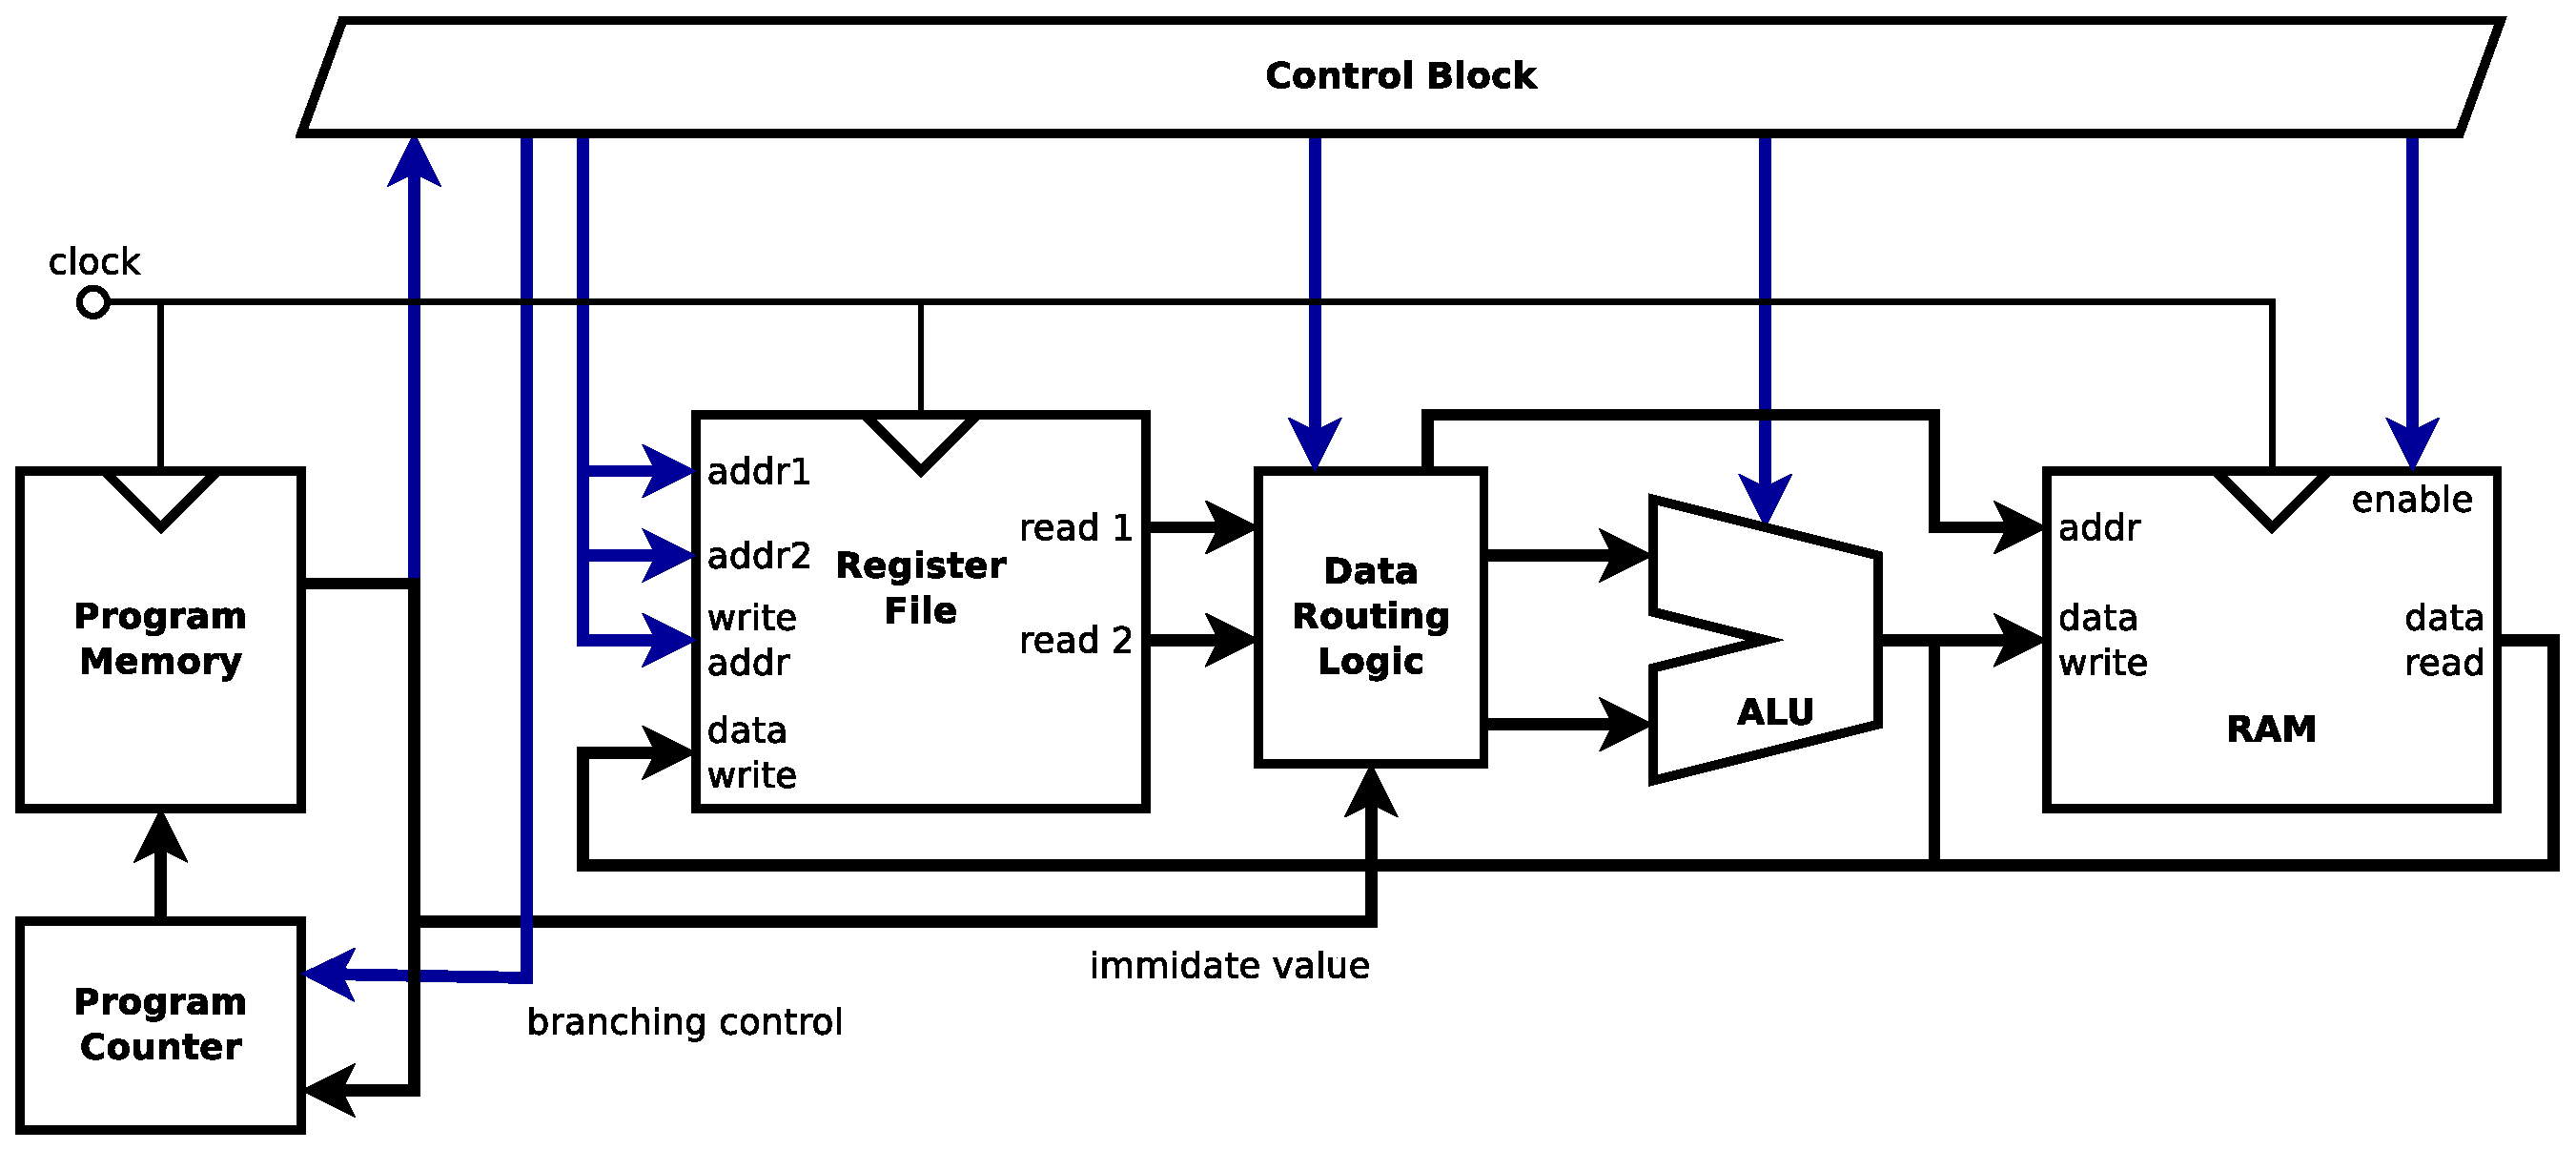
\includegraphics[width=\linewidth]{../resources/risc.eps}
	\caption{Abstract diagram of proposed RISC structure}
	\label{fig:risc_simple}
\end{figure*}

In this project, proposed RISC microarchitecture is mainly based on MIPS microachitecture \autocite{harris_harris_2013}. Figure \ref{fig:risc_simple} represents simplified diagram of proposed RISC processor. In this architecture, program data travels from program memory to the control block where instruction is decoded. Then control block further decides how data is directed in the datapath block. Such structure requires a complicated control block and additional data routing blocks. Depending on instruction, control block sets ALU, register file, memory operations and how data flows from one to other. Therefore, if non of blocks are bypassed, data can flow though every of these blocks, creating a log chain of combinational logic and increasing critical path. However this enables great flexibility allowing multiple operations to happen during single step, for example load value from register to memory, while address value is immediate offset by other register value using ALU. In order to increase performance of such processor, pipelining or multiple cores may be used.

\subsubsection{Pipelining}
\begin{multline}\label{eq:tc}
	\begin{split}
	T_c =& t_{pcq} + t_{ROM} + t_{register} + \\
	 	 & t_{routing} + t_{ALU} + t_{RAM} + t_{setup}
	\end{split}
\end{multline}

Equation \ref{eq:tc} shows maximum processor cycle period $T_c$ which depends on combinational logic delay of every logic block, flip-flop time of propagation from clock to output of synchronous sequential circuit $t_{pcq}$ and flip-flop setup time $t_{setup}$.

\begin{align}\label{eq:tcp}
	T_{cp} &= max \left( \begin{matrix}
	t_{pcq} + t_{ROM} + t_{setup},\\
	t_{pcq} + t_{register} + t_{setup},\\
	t_{pcq} + t_{ALU} + t_{setup},\\
	t_{pcq} + t_{RAM} + t_{setup}\\
	\end{matrix}\right)
\end{align}

Pipelinig separates each processor datapath block with a flip-flop. This changes combinational logic critical path this reducing cycle period. Pipelined processor cycle period $T_{cp}$ is represented in equation \ref{eq:tcp}. Such modification could technically increase clock frequency by 2 or 3 times.

Pipelining, however, introduces other design complications. Instructions that depend on each other, for example operation $R = A + B + C$ needs to be executed in two steps, $t = A + B$ and $R = t + C$. Second step is depends and previous step result. Therefore additional logic is required to detect such dependencies and bypass datapath stages, or stall pipelining. Furthermore, breaching would also require stalling, temporary saving datapath stage and restoring it if needed when branching is concluded, or further branch prediction logic. Such dependency and branching issue requires hazards prevention logic which increases processor complexity and required resources. 

\subsubsection{Multiple cores}

Multicore system is a solution to increase processor throughput by having multiple datapath and control logic instances, each running separate instructions. Cores share other resources such as RAM.

Multicore processor requires software adjustments as each processor core would execute separate programs. Therefore, some synchronisation between them is needed. A single additional core would also double the control and datapath blocks, substantially increasing resource requirements too. In addition, problems most often cannot be perfectly divided to parallel tasks due to some result dependencies between each task. Therefore, doubling processor core count would not likely result double the performance. 

\subsection{OISC Processor}

\begin{figure*}[t!]
	\centering
	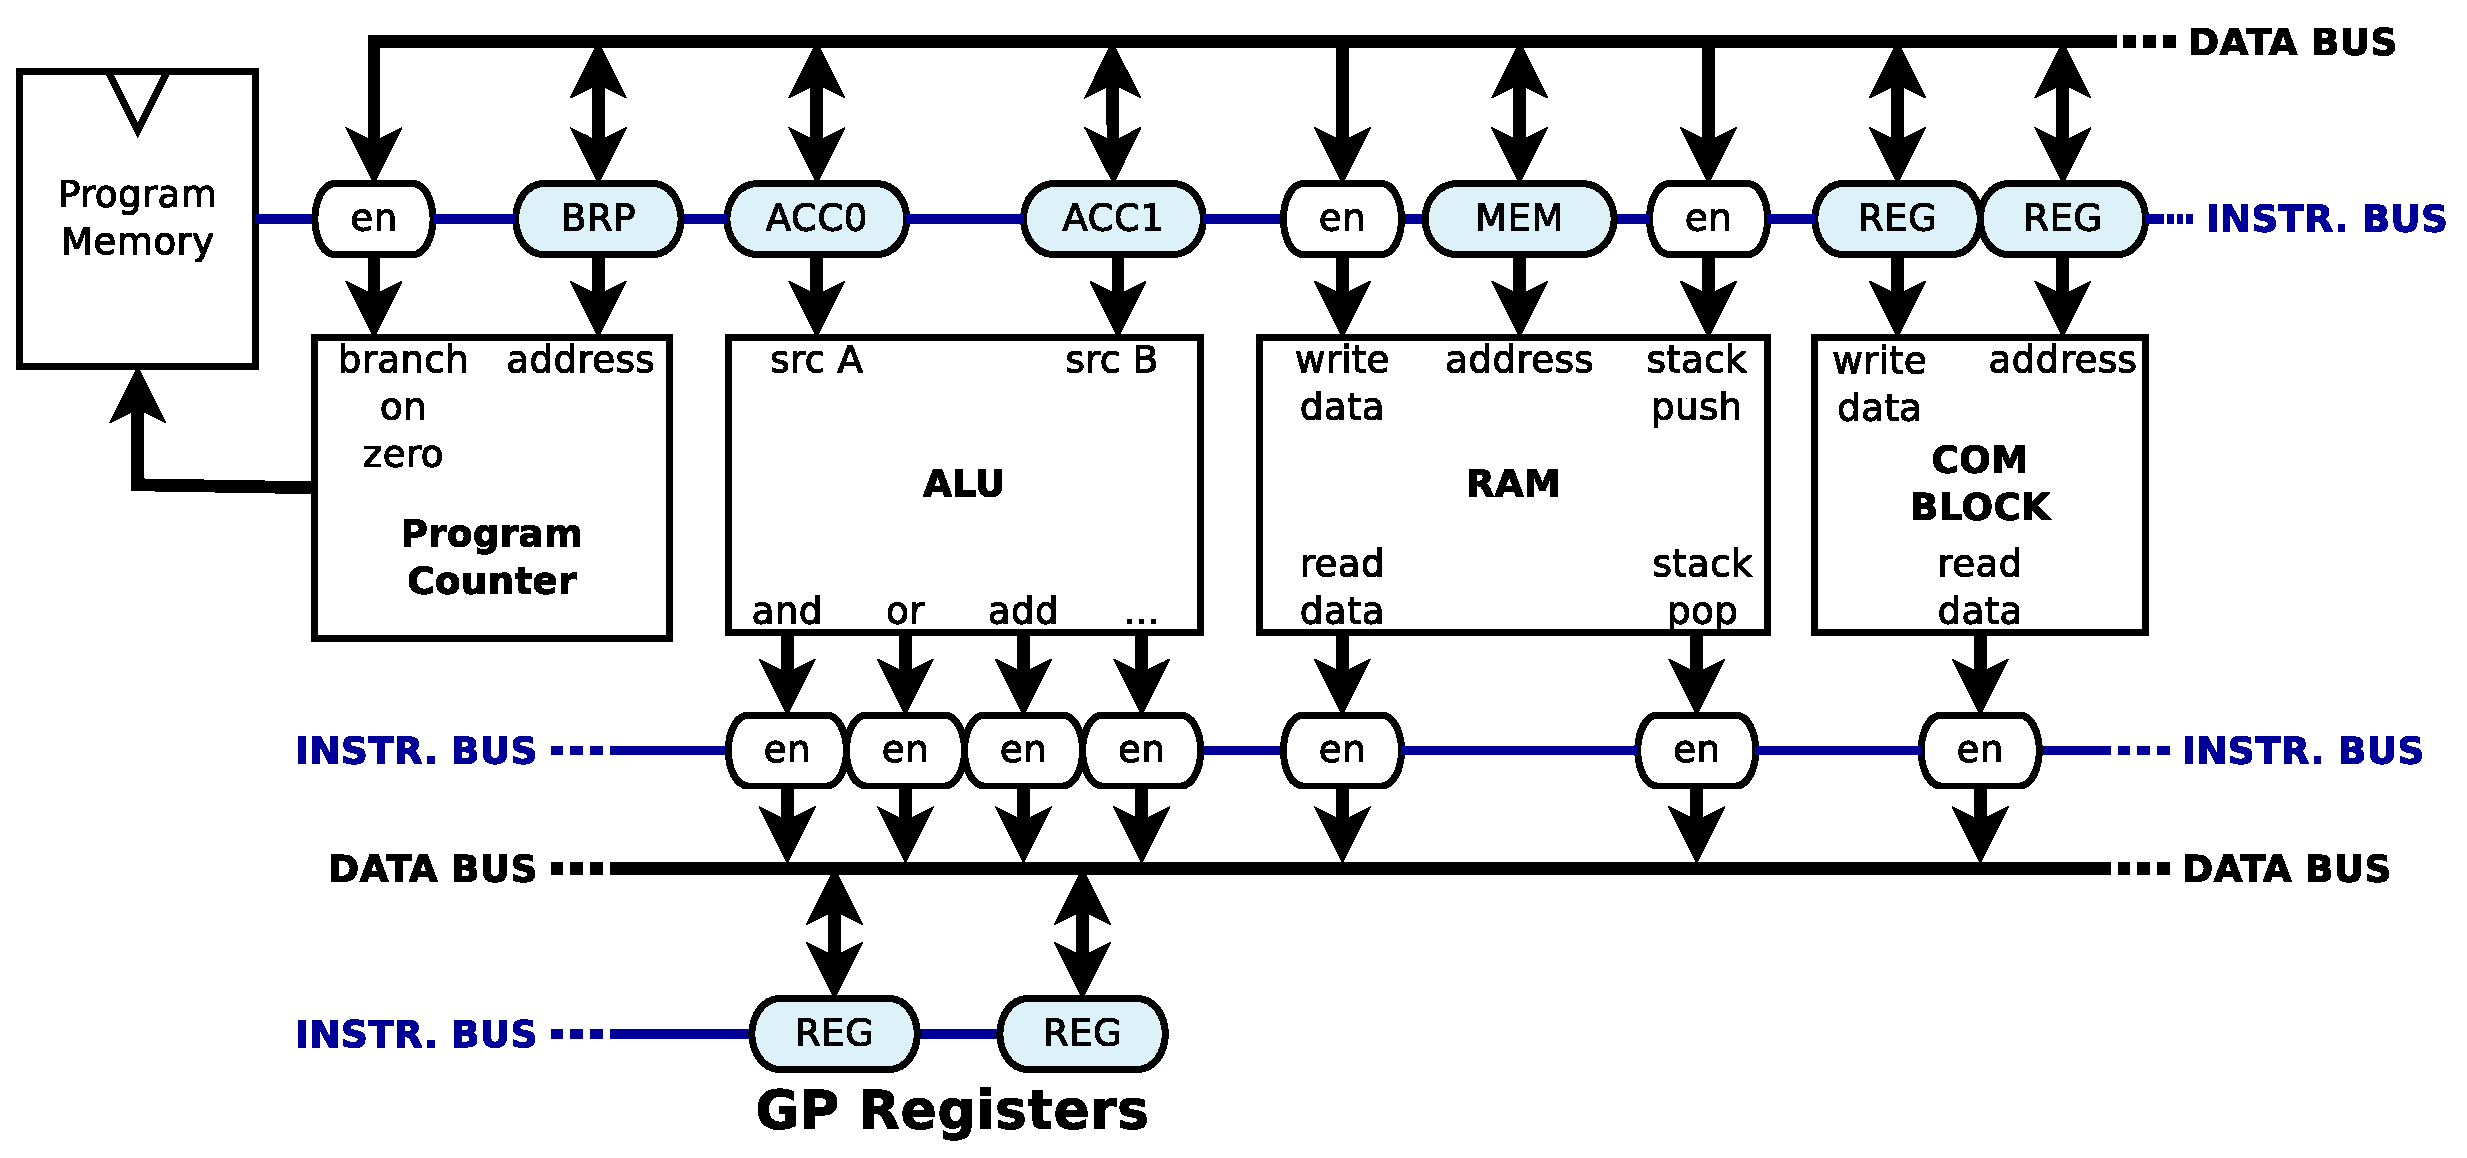
\includegraphics[width=\linewidth]{../resources/oisc.eps}
	\caption{Abstract diagram of proposed OISC structure}
	\label{fig:oisc_simple}
\end{figure*}

Figure \ref{fig:oisc_simple} represents simplified structure of OISC MOVE architecture. In simplest case, processor has a pair of buses - data and instruction. Instruction bus has source and destination address that connects two parts of processor via data bus. This mechanism allows data to flow around processor. Computation is accomplished by setting accumulators at destination addresses and taking computed values from source addresses. Other actions can be performed by at destination node for instance check value for branching or sending data to memory. 

\subsubsection{OISC Pipelining}
Maximum processor cycle period of such processor microarchitecture can be found in Equation \ref{eq:oisc_tc}. 

\begin{multline}\label{eq:oisc_tc}
	\begin{split}
t_{CL} &= max \left( \begin{matrix}
t_{register},\\
t_{ALU},\\
t_{RAM}\end{matrix}\right)\\
&\\
T_{cp} &= max \left( \begin{matrix}
t_{en} + t_{buf},\\
t_{pcq1}\end{matrix}\right) +\\
&\qquad\qquad+ t_{pcq2} + t_{CL} + t_{setup}
	\end{split}
\end{multline}


Where $t_{en}$ is period to check if instruction bus address match, $t_{buf}$ is period for source buffer to output value to data bus, $t_{pcq2}$ is propagation period for program memory, $t_{CL}$ represents longest propagation period though a logic block, $t_{setup}$ is setup time inside logic block. $t_{pcq1}$ and $t_{pcq2}$ are clock to output delay for sequential logic connecting logic block buffer and memory connecting instruction bus, respectively. 

\subsection{Predictions}

Comparing to RISC, OISC maximum processor cycle period is almost equivalent to pipelined RISC, just including 
enable, buffer and additional ROM delays: $max \left( t_{en} + t_{buf}, t_{pcq1}\right)$. In most cases $t_{CL}$ is going to dominant value, meaning that OISC should have higher $T_{cp}$ to non-pipelined RISC, or equivalent to pipelined RISC architectures. 

Further more, due to the nature of processor, no additional hazard prevention logic is needed making this much simpler design. In addition, $t_{CL}$ pipelining can be introduced to logic blocks that has high propagation delay. For instance, multiplication in ALU could be pipelined in two sections, when setting ALU accumulators software could be designed in such way to retrieve multiplied result only after two cycles. This can further reduced required logic circuit.

\subsubsection{Execution time}
OISC requires take extra steps to perform basic functions to set ALU, branch or memory operations need setting accumulator values. A single data-instruction bus OISC expected to be slower to execute the same task. 

\subsubsection{Instruction Space}
RISC has fairly compact instructions as single instruction can carry a small opcode, register value and immediate value. OISC has a bigger overhead as it can only set source and destination address which can carry only single operation, register or immediate value. Therefore it is expected OISC taking more instruction space for same function.

\subsubsection{Resources}
OISC does not have a control block which contains how data travel in datapath. It also does not have multi-adress register file and further routing logic. This indicate that OISC should require less logic elements to implement a processor. This should also result in lower power consumption. 
%There are many papers looking into application specific TTAs. 
	\vfill\pagebreak
	
	\section{Technical Method}\label{sec:methods}
	% !TeX root = index.tex
\iffalse
This chapter lays out your approach. 
What did you actually do to reach your goal, or attempt to reach your goal? 
What equipment did you use? 
How did you build the device? 
How did you set up the simulation: what mesh values, for example, did you use?

Provide enough detail that your work can be duplicated by someone else.
Be precise and use the correct units.
\fi


This section describes methods and design choices used to construct two processors.

\subsection{Machine Code}\label{subsec:machine_code}

\subsubsection{RISC Machine Code}
As the aim of instruction size to be as minimal as possible, RISC instruction decided to be 8bits with optional additional immediate value from 1 to 3 bytes. Immediate values are explained in section \ref{subsec:imm_values}.

Decision was made to have instruction compose of operation code two operands - source/destination and source, which is similar to x86 architecture rather than MIPS. Three possible combinations of register address sizes are possible in such case from one to three bits. Two was selected as it allow having four general purpose registers which is sufficient for most applications, and allow four bits for operation code - allowing up to 16 instructions. 

Due to small amount of possible operation codes and not all instructions requiring two operands (for example \texttt{JUMP} instruction may not need any operands or could use one operand to have address offset), other two type instructions are added to the design - with one and zero operands. See figure \ref{fig:risc_machinecode}. This enabled processor to have 45 different instructions while maintaining minimal instruction size. Final design has:
\begin{description}[labelindent=1cm, labelsep=1em]
	\item[$\bullet$ \textbf{8 }]  2-operand instructions
	\item[$\bullet$ \textbf{32}]  1-operand instructions
	\item[$\bullet$ \textbf{5 }]  0-operand instructions
\end{description}
Full list of RISC instructions are listed in table \ref{tab:risc_instructions} in \nameref{sec:appendix} section.

\begin{blockpage}
\begin{gather*}
\scalebox{0.8}{2 operands:}~
\underbrace{
	\colorbox{c1}{0}\,
	\colorbox{c1}{1}\,
	\colorbox{c1}{2}\,
	\colorbox{c1}{3}
}_\text{op. code}
\underbrace{
	\colorbox{c2}{4}\,
	\colorbox{c2}{5}
}_\text{dst.}
\underbrace{
	\colorbox{c3}{6}\,
	\colorbox{c3}{7}
}_\text{src.}
\\
\scalebox{0.8}{1 operand:}~
\underbrace{
	\colorbox{c1}{0}\,
	\colorbox{c1}{1}\,
	\colorbox{c1}{2}\,
	\colorbox{c1}{3}
}_\text{op. code}
\underbrace{
	\colorbox{c2}{4}\,
	\colorbox{c2}{5}
}_\text{dst.}
\underbrace{
	\colorbox{c1}{6}\,
	\colorbox{c1}{7}
}_\text{op. c.}\\
\scalebox{0.8}{0 operands:}~
\underbrace{
	\colorbox{c1}{0}\,
	\colorbox{c1}{1}\,
	\colorbox{c1}{2}\,
	\colorbox{c1}{3}\,
	\colorbox{c1}{4}\,
	\colorbox{c1}{5}\,
	\colorbox{c1}{6}\,
	\colorbox{c1}{7}
}_\text{operation code}
\end{gather*}
\begin{center}
\captionof{figure}{\textit{RISC instructions composition. Number inside box represents bit index. Destination (dst.) bits represents of source and destination register address.}}
\label{fig:risc_machinecode}
\end{center}
\end{blockpage}

\subsubsection{OISC Machine Code}

As OISC requires only a single instruction, composition of instruction mainly requires two parts - source and destination. To allow higher instruction flexibility a immediate bit has been added to replace source address by immediate value. Composition of finalised machine code is shown in figure \ref{fig:oisc_machinecode}. 

\begin{blockpage}
\begin{gather*}
\underbrace{
	\colorbox{c1}{0}
}_\text{imm.}
\underbrace{
	\colorbox{c2}{1}\,
	\colorbox{c2}{2}\,
	\colorbox{c2}{3}\,
	\colorbox{c2}{4}\,
}_\text{destination}
\underbrace{
	\colorbox{c3}{5}\,
	\colorbox{c3}{6}\,
	\colorbox{c3}{7}\,
	\colorbox{c3}{8}\,
	\colorbox{c3}{9}\,
	\colorbox{c3}{10}\,
	\colorbox{c3}{11}\,
	\colorbox{c3}{12}
}_\text{source}
\end{gather*}

\begin{center}
\captionof{figure}{\textit{OISC instruction composition. Number inside box represents bit index.}}
\label{fig:oisc_machinecode}
\end{center}
\end{blockpage}

Decision was made to have source address to be eight bits to allow it be replaced with immediate value. Destination address was chosen to be as minimal as possible, leaving only four bits or 16 possible destinations. Final design has \textbf{15} destination and \textbf{41} source addresses. This is not the most space efficient design as 41 source addresses would require only six bits for address, wasting two bits every time non-immediate source is used.

Full list of OISC sources and destinations are listed in table \ref{tab:oisc_instructions} in \nameref{sec:appendix} section.

\begin{landscape}
	\subsection{Data flow} \label{sec:dataflow}
	\subsubsection{RISC Datapath} \label{subsec:datapath}
	\begin{figure}[h!]
		\centering
		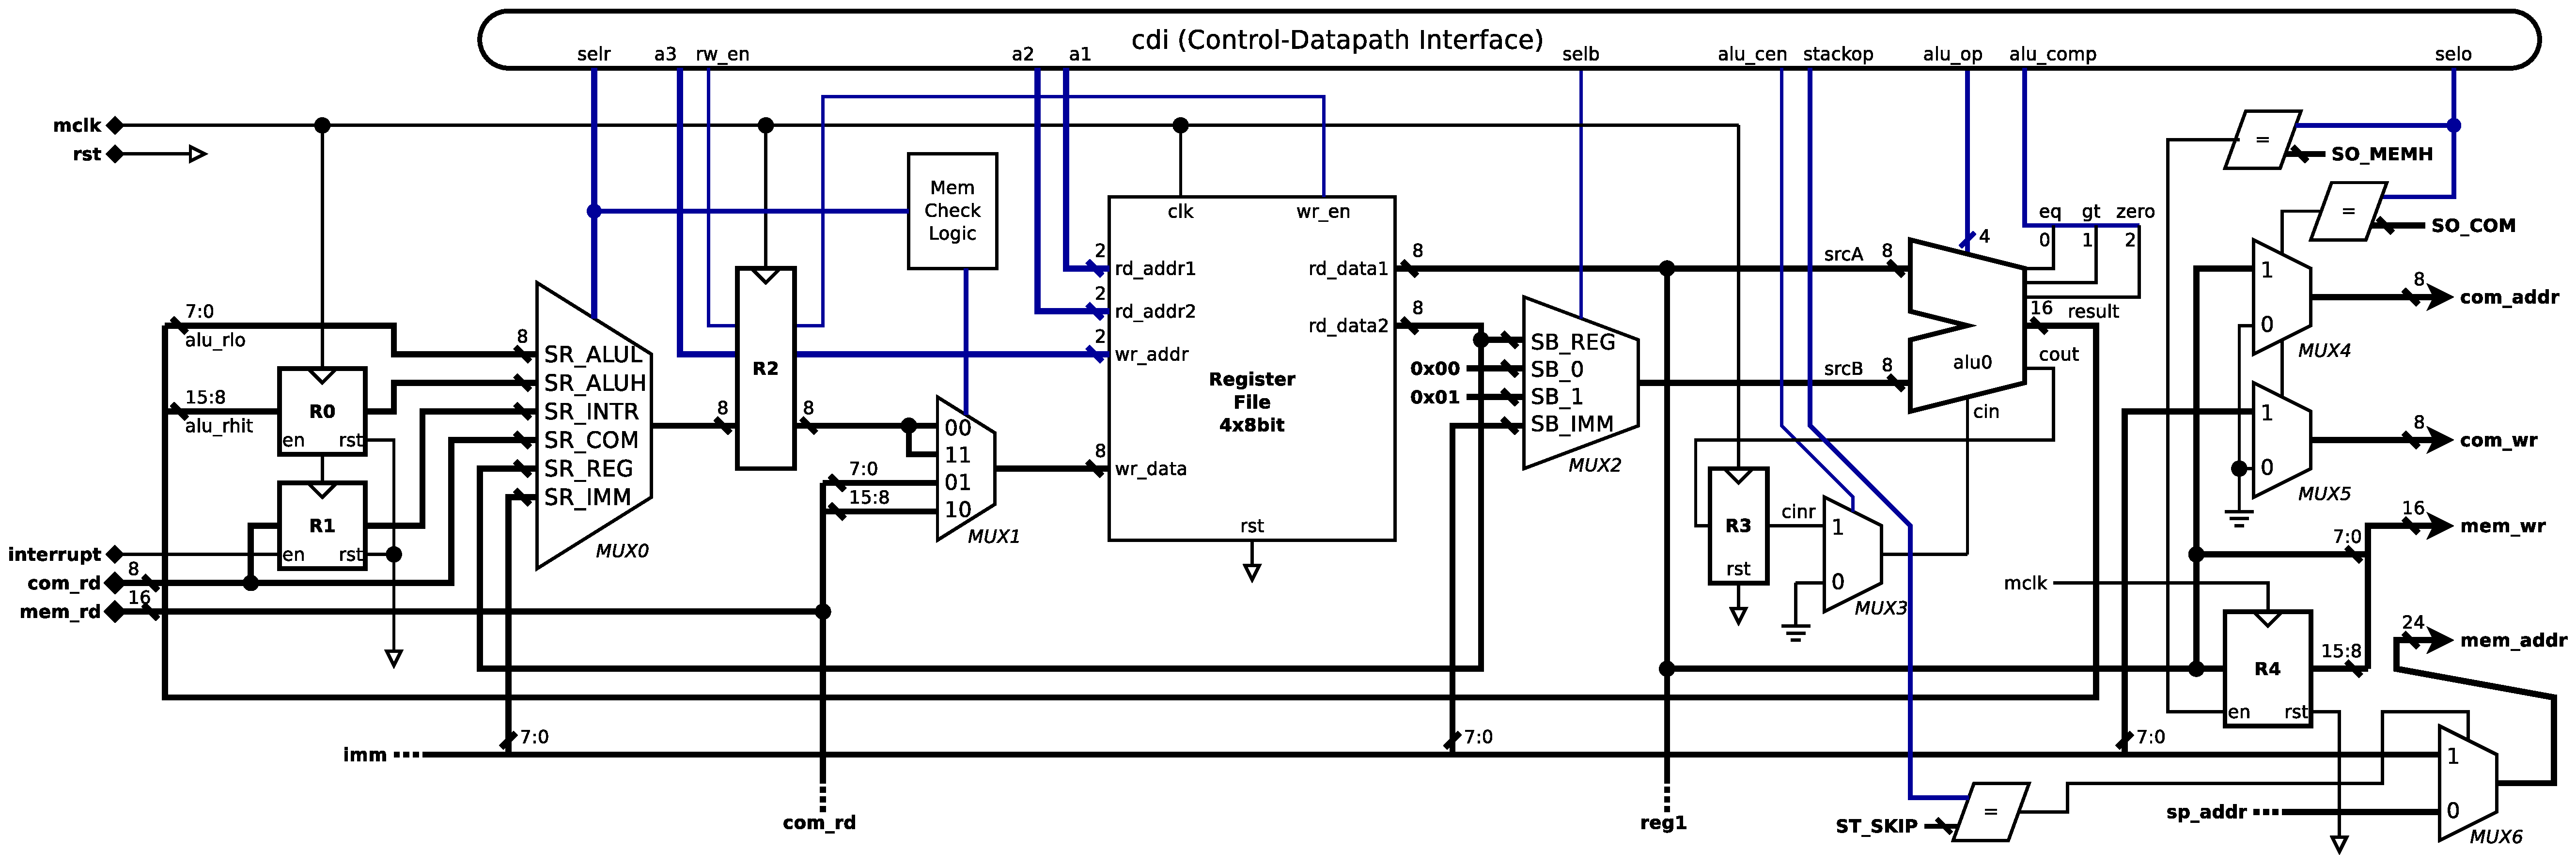
\includegraphics[width=\linewidth]{../resources/datapath.eps}
		\caption{Digital diagram of RISC datapath}
		\label{fig:datapath}	
	\end{figure}
	
	Figure \ref{fig:datapath} above represents partial RISC datapath. This diagram can be extends to Program counter, Stack pointer and Immediate Override logics are represented in figures \ref{fig:risc_pc}, \ref{fig:risc_stack} and \ref{fig:risc_imo} respectively. CDI (Control-Data Interface) is HDL concept that connects datapath and control unit. Immediate value to datapath is provided by IMO block described in section \ref{subsec:imo}.\\
	Data to register file is selected and saved with \textit{MUX0}. This data is delayed 1 cycle with \textit{R2} to match timing that of data is taken from memory. If \texttt{LWLO} or \texttt{LWHI} is executed, \textit{MUX1} select high or low byte from memory to read. To compensate for timing as value written to register file is delayed by 1 cycle, register file has internal logic that outputs \textit{wr\_data} to \textit{rd\_data1} or/and  \textit{rd\_data2} immediately if \textit{wr\_en} is high and \textit{rd\_addr1} or/and \textit{rd\_addr2} matches \textit{wr\_addr}. \\
\end{landscape}
\textit{MUX2} allows override ALU source B, \textit{R3} and \textit{MUX3} enables control unit to enable ALU carry in allowing multi-byte number addition/subtraction. This function is not fully implemented yet.\textit{MUX4} and \textit{MUX5} allows to send data to COM block with \texttt{COM} instruction, if other instruction performed then \textit{0x00} byte for COM address and data is sent, indicating no action. Data is stored in memory only with \texttt{SWLO} instruction writing to high byte whatever is stored in \textit{R4} buffer. This buffer can be written to using \texttt{SWHI} instruction. \textit{MUX6} selects memory address value from \textit{imm} or stack pointer.

\subsubsection{OISC Datapath} \label{subsec:oisc_cells}

OISC datapath only consists of instruction and data buses, and small circuit that connect them to logic blocks that process the data. These logic blocks can represent ALU operation combinational logic, or any other part of a processor.

Figure \ref{fig:oisc_cell_in} represents common destination circuit. It checks if particular block destination matches one on instruction bus, then enables latch and also sets flag to further logic. 
\begin{colfigure}
	\centering
	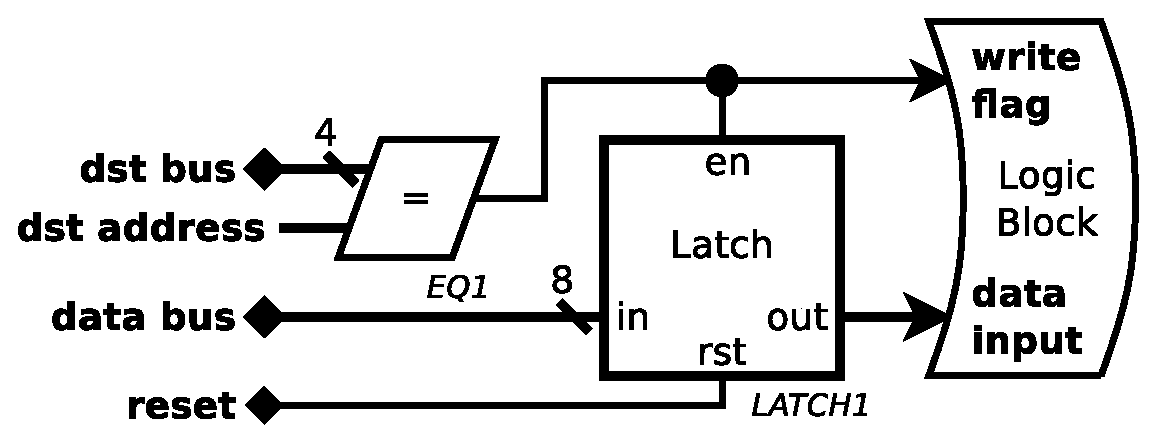
\includegraphics[width=\linewidth]{../resources/oisc_cell_in.eps}
	\captionof{figure}{OISC processor data bus to destination connection logic}
	\label{fig:oisc_cell_in}
\end{colfigure}

Similarly Figure \ref{fig:oisc_cell_out} represents source circuit connecting output of logic block. As logic block may only involve combinational logic a register is placed at the output of it. Buffer is used to connect data in register to data bus. This ensures that only one bus driver is present, ensuring do data collision. 

\begin{colfigure}
	\centering
	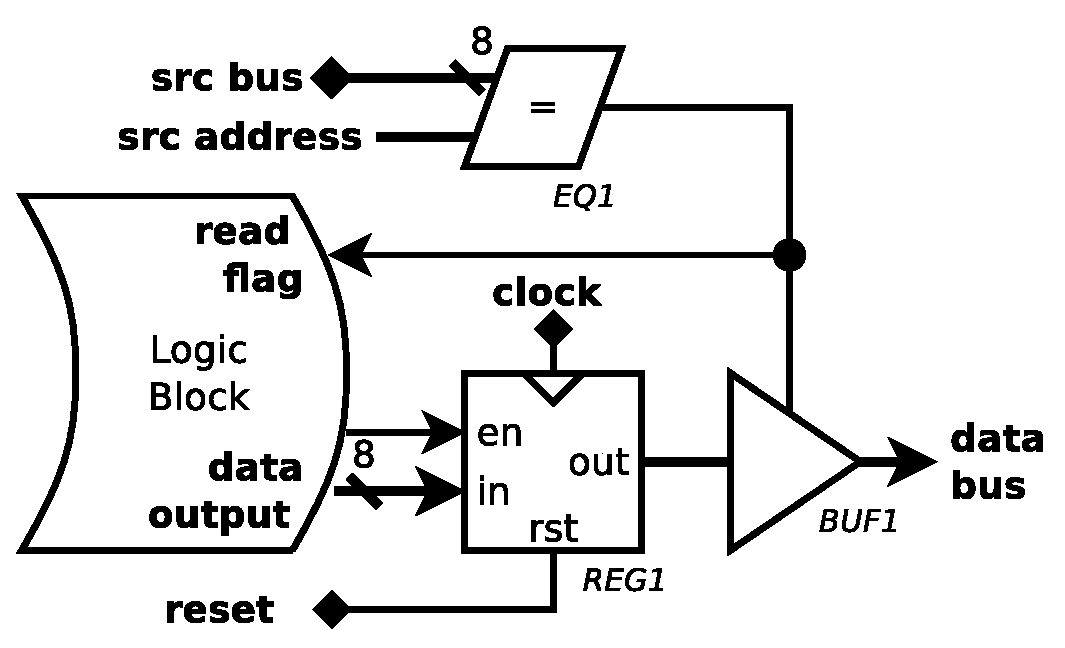
\includegraphics[width=\linewidth]{../resources/oisc_cell_out.eps}
	\captionof{figure}{OISC processor data bus to source connection logic}
	\label{fig:oisc_cell_out}
\end{colfigure}

The general timing is designed so that the information at the source is immediately ready in data bus at rise of the processor clock. The source is connected to the destination connection where combinational logic is present. 

\subsubsection{OISC Datapath Implementation Problems} \label{subsec:oisc_cell_issue}

The complete implementation using latches for destination was not successful. Latches did not operate correctly when synthesised on FPGA. This issue might be caused by some timing problem between some source and destination logic combination. Exact cause was not resolved.

As a quick solution, latches at destination has been replaced with a clocked register that is triggered at opposite to source register clock edge (negative). This resolved this issue, however it effectively reduce period that data can propagate though logic blocks between source and destination by two.

\subsection{Stack} \label{subsec:stack}
This section describes RISC and OISC dedicated logic for stack pointer control. Stack pointer starts from the highest memory address value and "stacks" to lower memory address values. Both designs were simplified to only operate on two byte addresses, meaning that stack pointer has a constant \texttt{0xFF} value at least significant byte. 


\subsubsection{RISC Stack}
RISC processor implements the stack pointer that is used in \texttt{PUSH}, \texttt{POP}, \texttt{CALL} and \texttt{RET} instructions. The stack pointer's initial address starts at the highest memory address (\texttt{0xFFFF}) and subtracts 1 when data is put to stack. Figure \ref{fig:risc_stack} represents the logic diagram for stack pointer. Note that the stack is only 16bit in size and the most significant byte is set to \texttt{0xFF}. The stack pointer circuit also supports \textit{pc\_halted} signal from program counter to prevent the stack pointer from being added by 1 twice during \texttt{RET} instruction. 

One of the problems with the current stack pointer implementation is 8bit data stored in 16bit memory address, wasting a byte. This can be avoided by adding a high byte register, however then it would cause problems when a 16bit program pointer is stored with \texttt{CALL} instruction. This can still be improved with a more complex circuit, or by using memory cache with 8bit data input. However with current implementation this does not affect processor comparison, it only increases stack size in memory.

\begin{figure*}
	\centering
	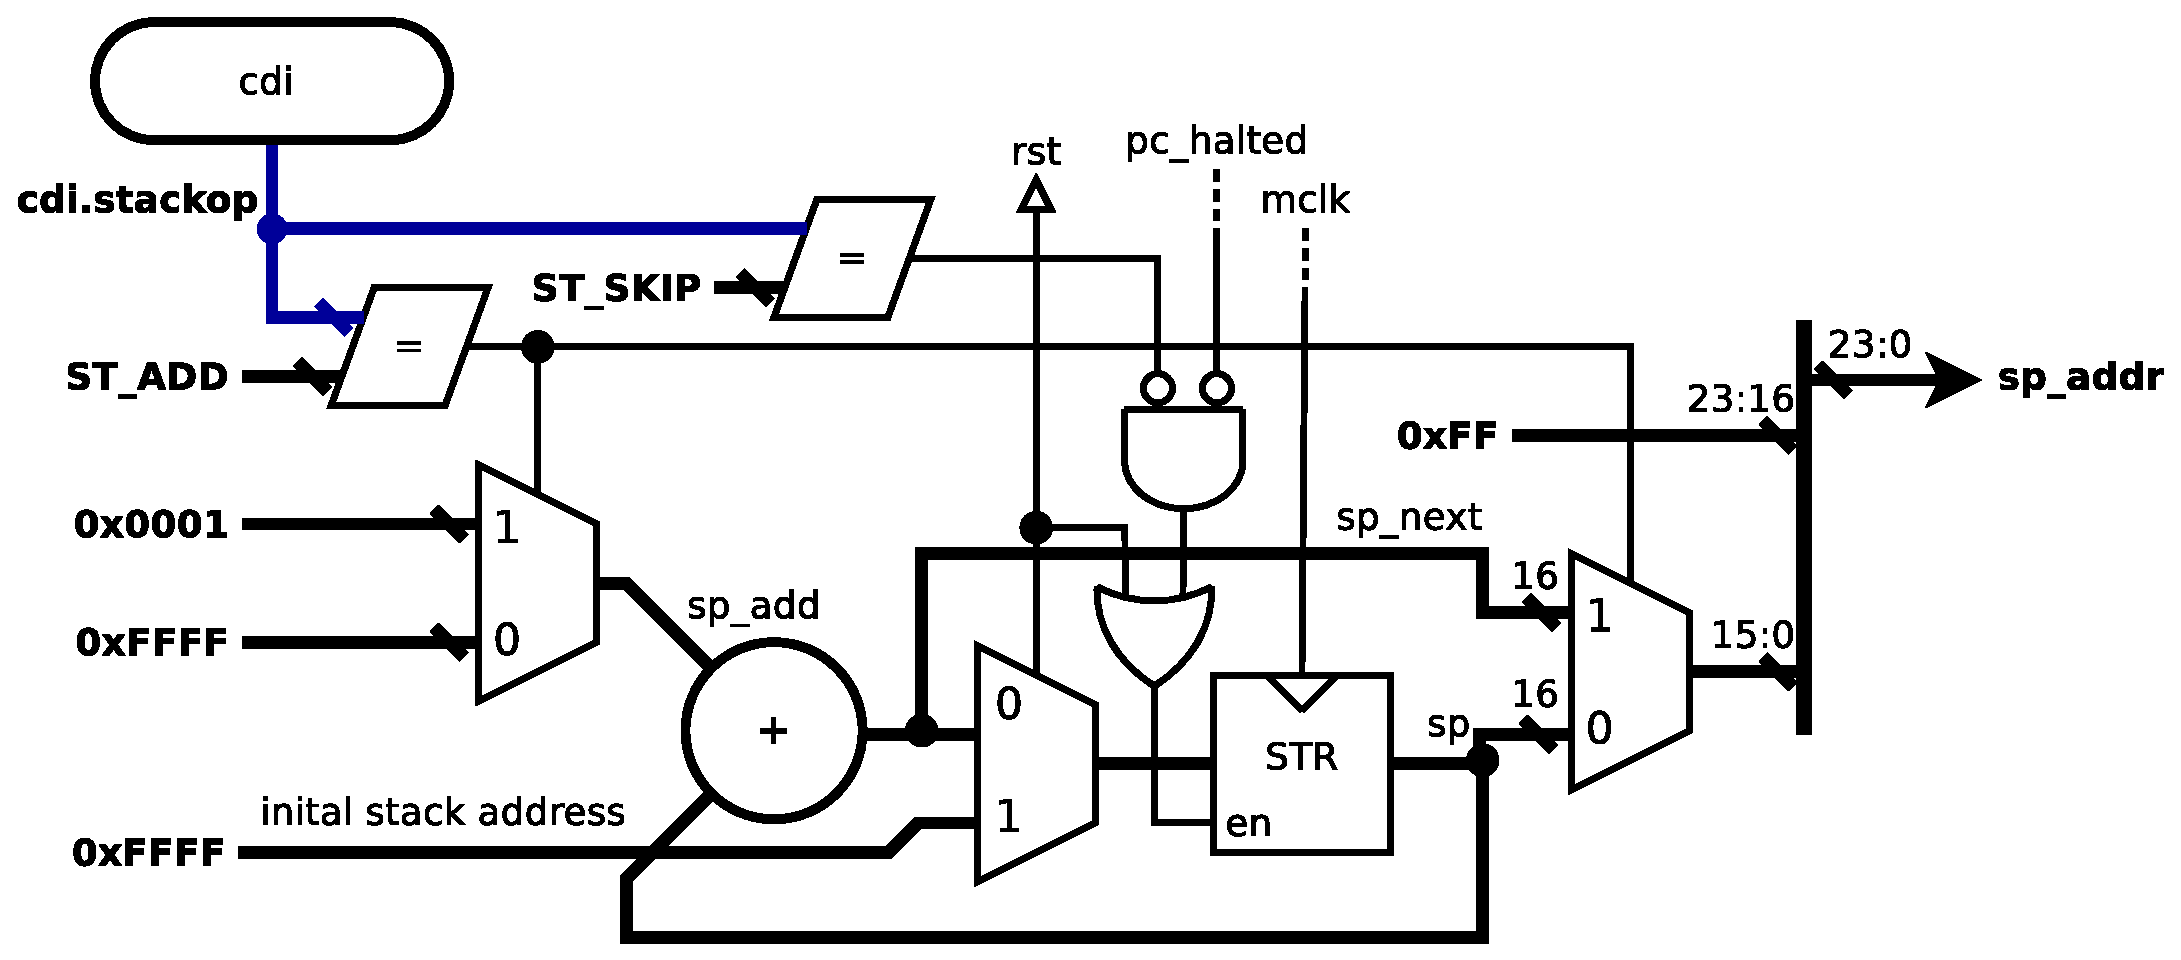
\includegraphics[scale=0.4]{../resources/risc_stack.eps}
	\caption{Digital diagram of RISC stack pointer logic}
	\label{fig:risc_stack}
\end{figure*}

\subsubsection{OISC Stack}

Stack pointer in OISC is very similar to RISC. In basic operation, when reset, push or pop flags are set, it changes the state of stack pointer by adding or subtracting its value by one, or resetting it to default. Logic diagram is shown in Figure \ref{fig:oisc_stack}
\begin{figure*}[b]
	\centering
	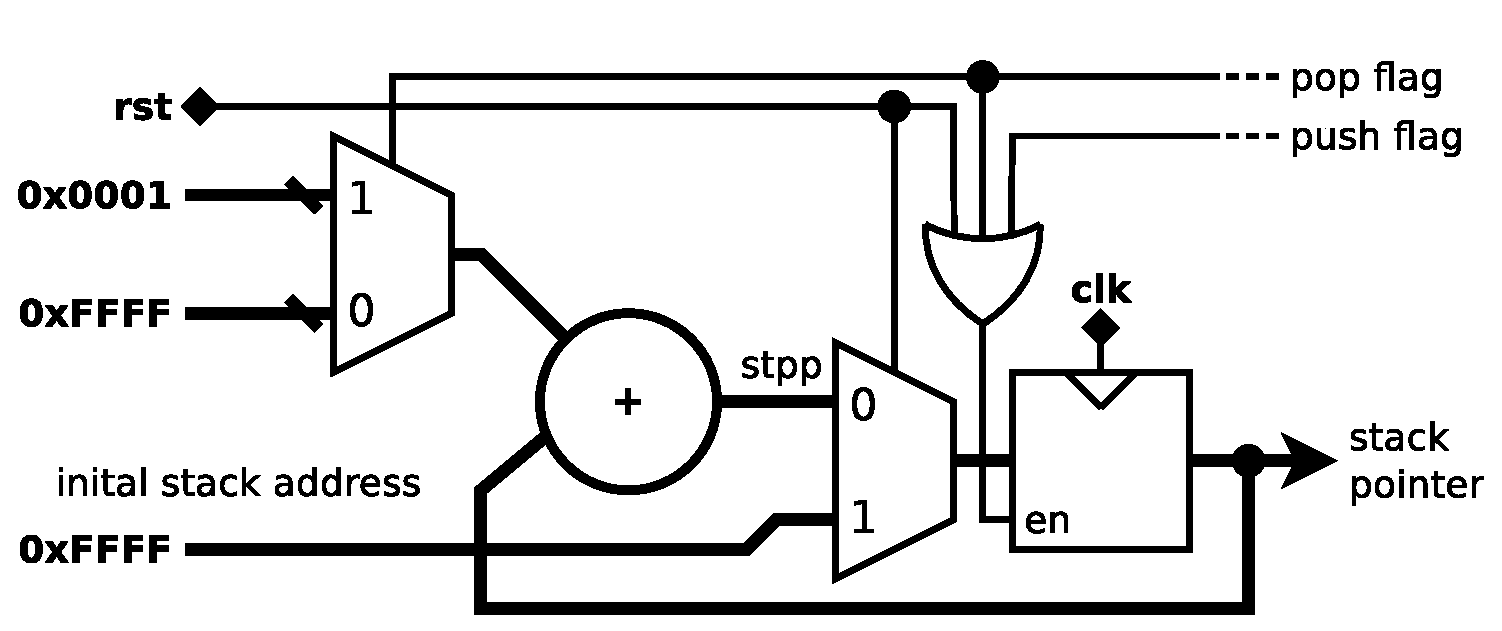
\includegraphics[scale=0.4]{../resources/oisc_stack.eps}
	\caption{Digital diagram of OISC stack pointer logic}
	\label{fig:oisc_stack}
\end{figure*}

Logic diagram of stack control unique to OISC processor is shown in Figure \ref{fig:oisc_stack_2}. Push and pop flags are taken from source and destination logic. A cached value of last stored value is kept, so that it would be immediately available on source request. Pop flag is delayed by one cycle which ensures that once popped, lower stack value is written to cache during next cycle.
\begin{figure*}
	\centering
	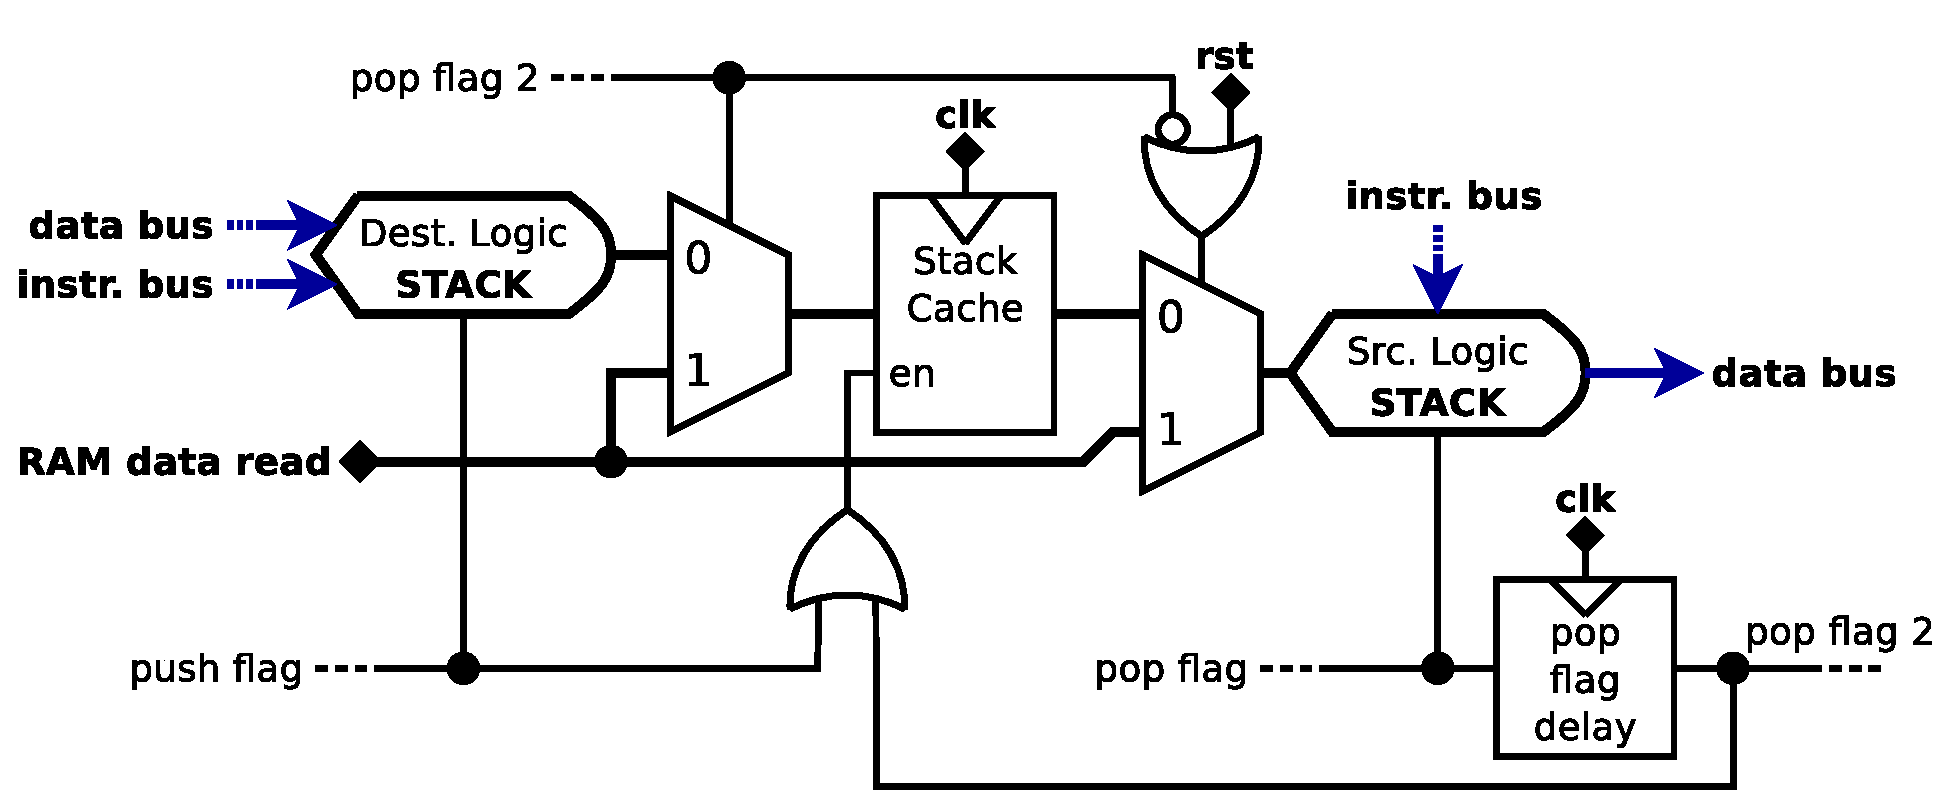
\includegraphics[scale=0.4]{../resources/oisc_stack_2.eps}
	\caption{Digital diagram of OISC stack control logic}
	\label{fig:oisc_stack_2}
\end{figure*}

\subsection{Program Counters} \label{subsec:pc}
In this subsection, program counter and their differences will be described.

\subsubsection{RISC Program Counter}

\begin{figure*}[h!]
	\centering
	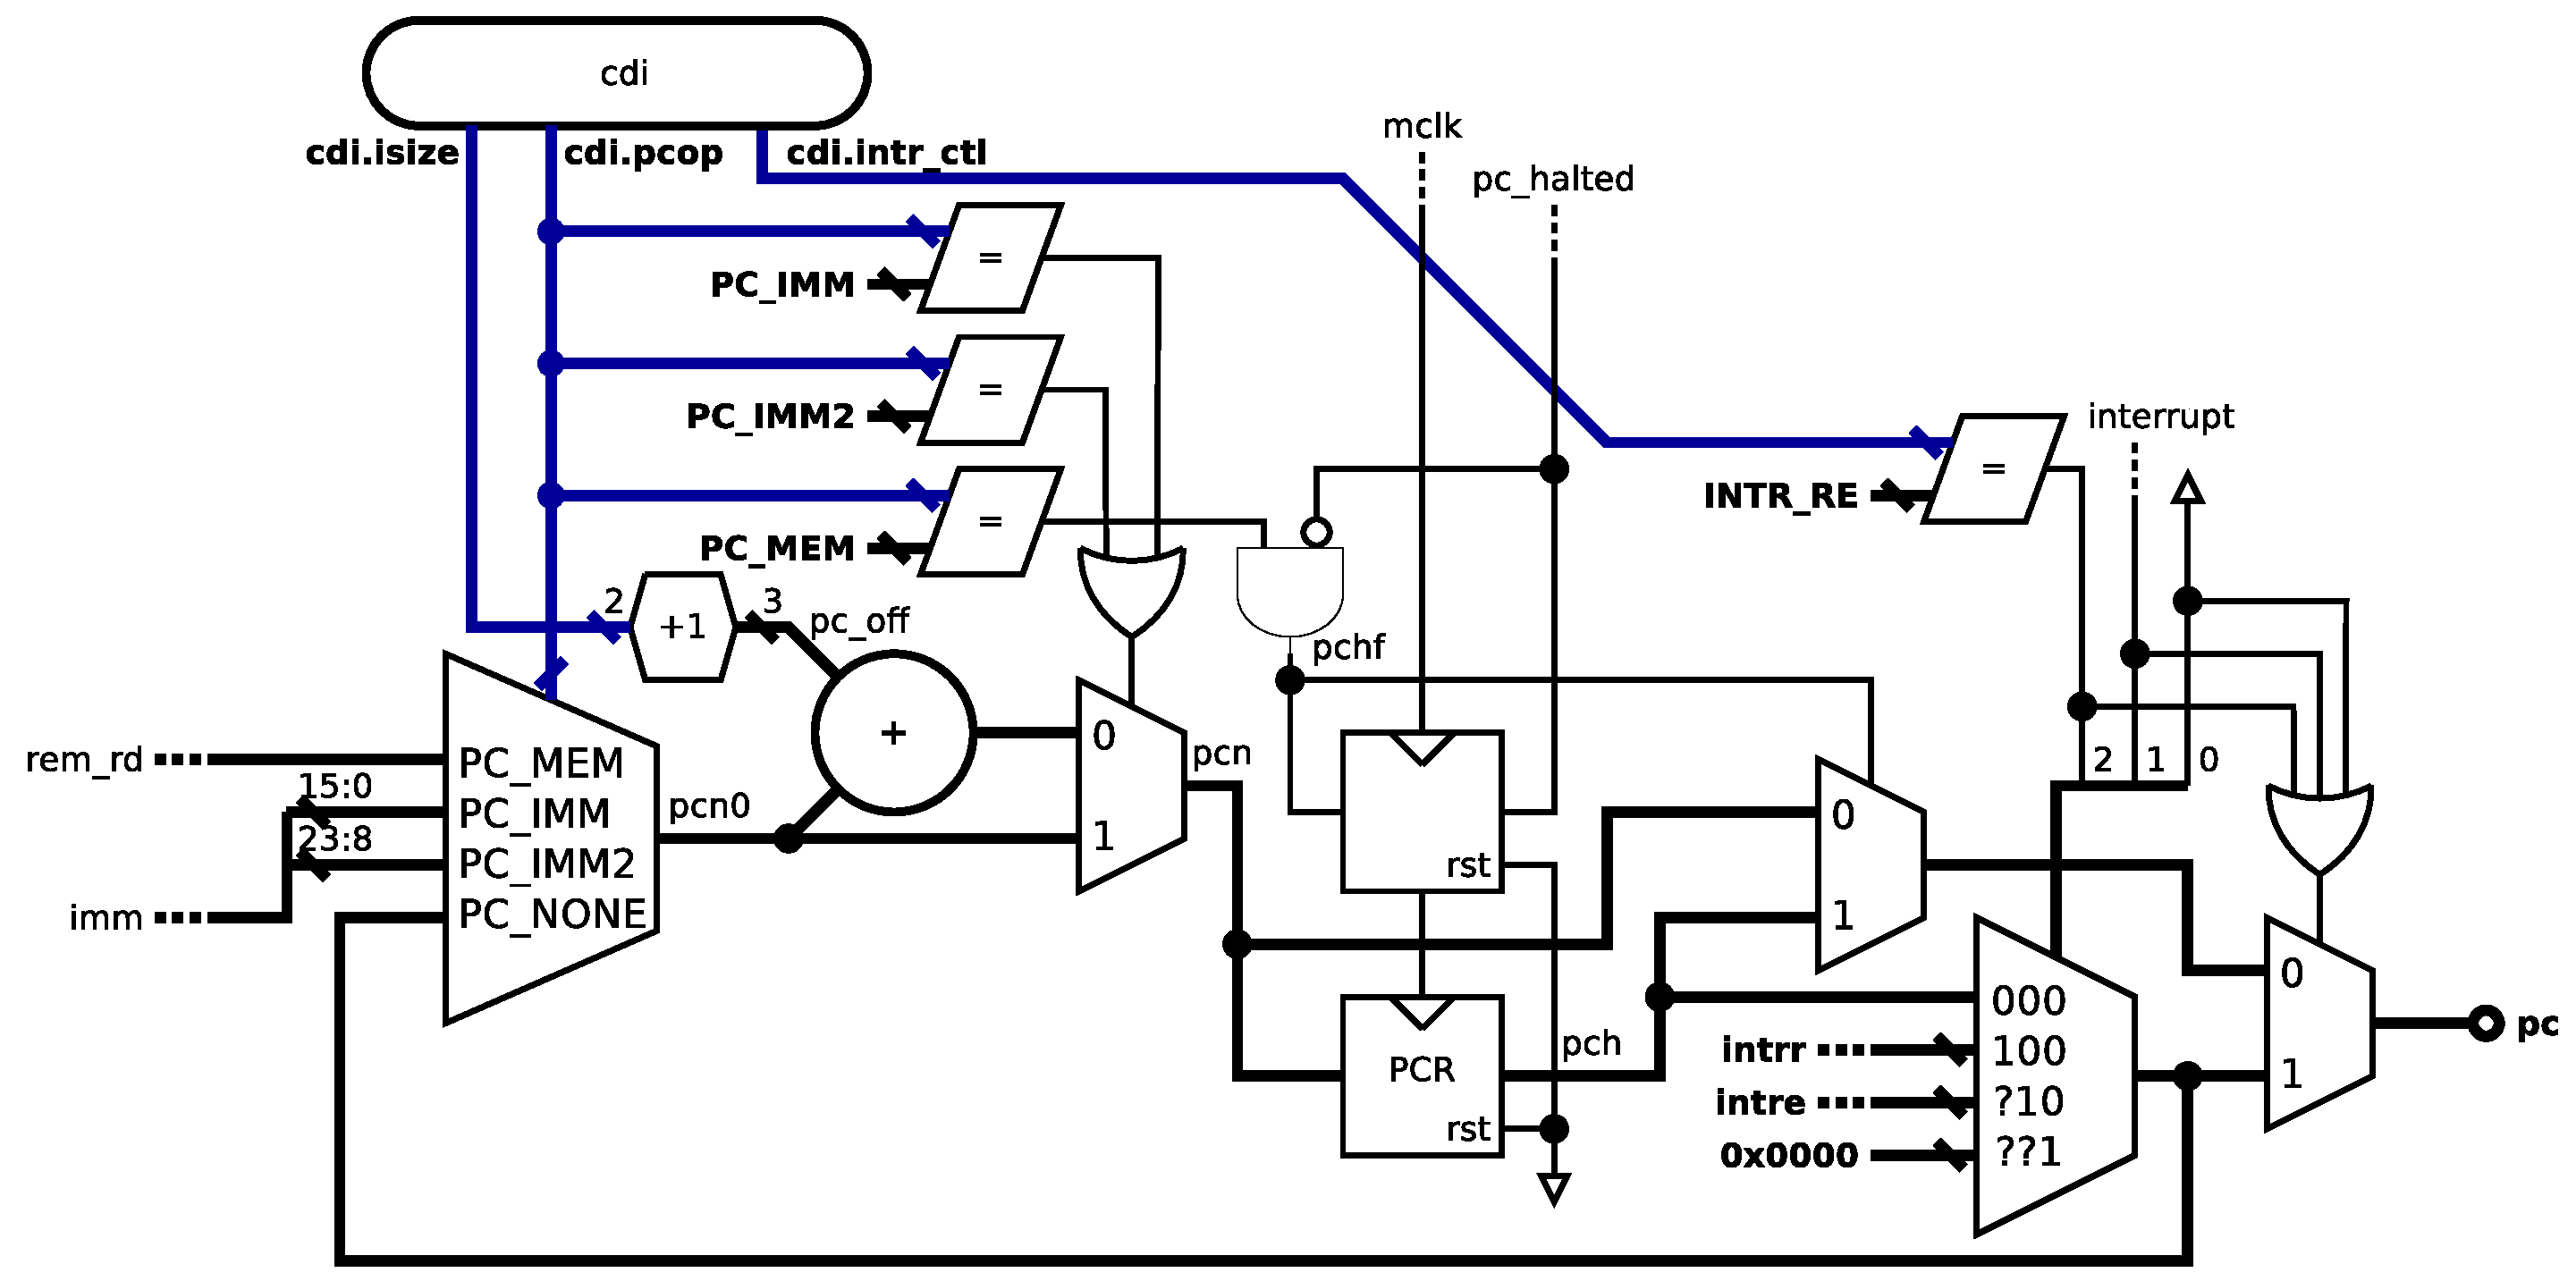
\includegraphics[width=\linewidth]{../resources/risc_pc.eps}
	\caption{Digital diagram of RISC program counter}
	\label{fig:risc_pc}
\end{figure*}

Figure \ref{fig:risc_pc} represents the digital diagram for program counter. There are a few key features about this design: it can take values from memory for \texttt{RET} instruction; immediate value (\textit{PC\_IMM2} is shifted by 1 byte to allow \texttt{BEQ}, \texttt{BGT}, \texttt{BGE} instructions as first immediate byte used as ALU source B); can jump to interrupt address; produces \textit{pc\_halted} signal when memory is read (\texttt{RET} instruction takes 2 cycles, because cycle one fetches the address from stack and second cycle fetches the instruction from the instruction memory).

\subsubsection{OISC Program Counter}\label{subsec:oisc_pc}
 
 OISC program counter is much simpler than RISC, as it does not have variable length instruction, delay flags instructions, or logic for selecting branch source address. 
 
\begin{colfigure}
	\centering
	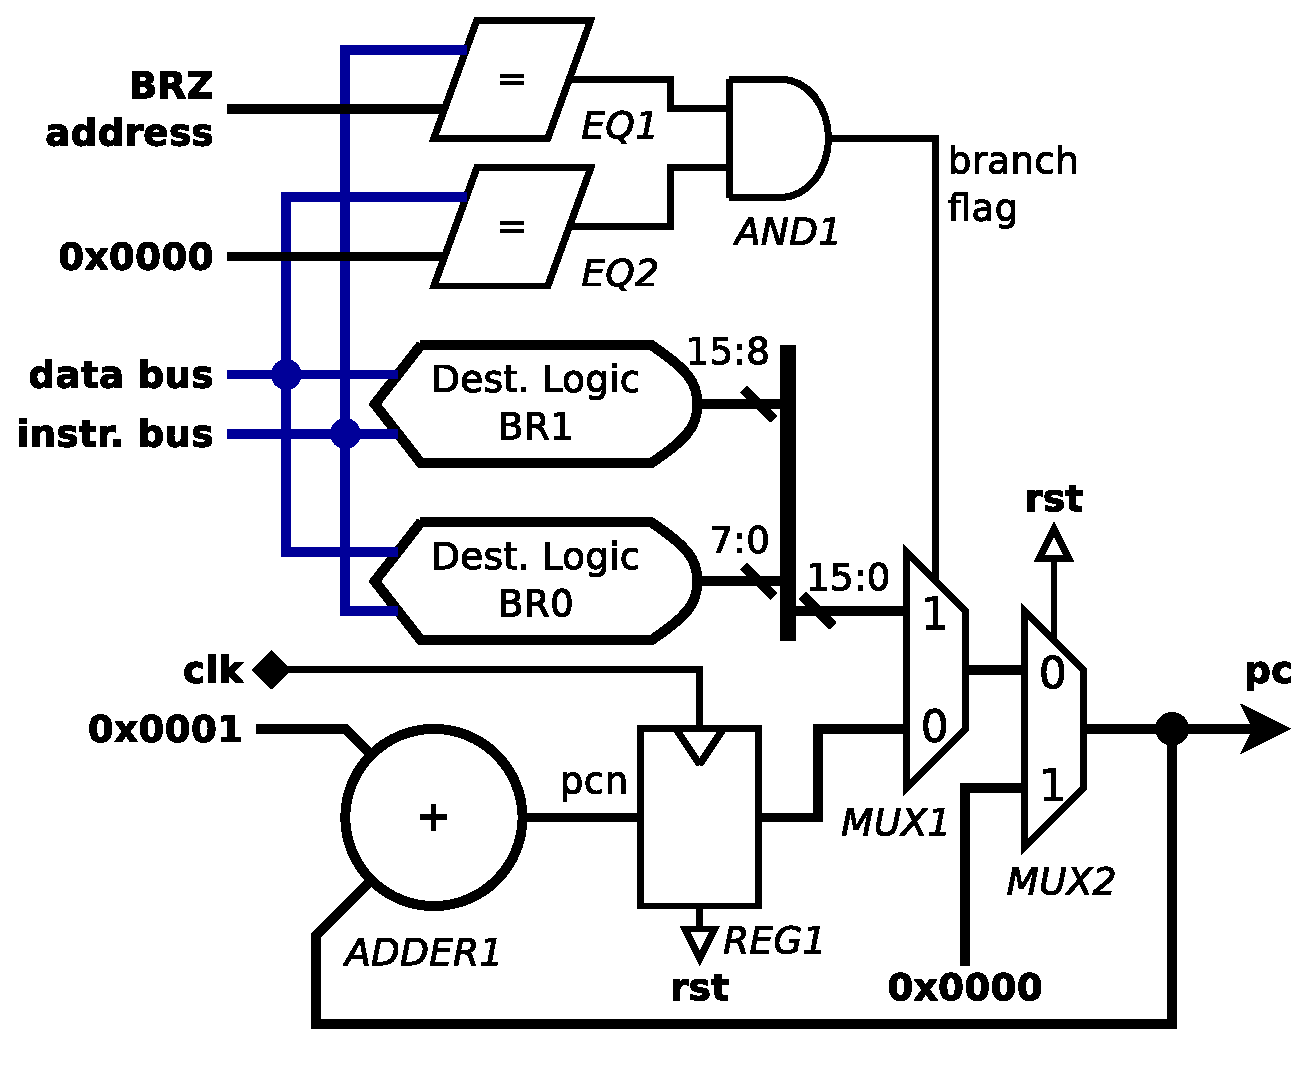
\includegraphics[width=\linewidth]{../resources/oisc_pc.eps}
	\captionof{figure}{Digital diagram of OISC program counter}
	\label{fig:oisc_pc}
\end{colfigure}

Looking at Figure \ref{fig:oisc_pc} bottom, the basic operation is to just add one to previous program counter with \textit{ADDER1} and \textit{REG1}, reset it to zero at reset with \textit{MUX2}. Two destination logic blocks are used as accumulators to store branch address. Once instruction with BRZ destination is executed, \textit{EQ2} check if data bus value is zero, which enables \textit{MUX1} and overrides program counter to address stored in \texttt{BR0} and \texttt{BR1} accumulators. Unlike in RISC however, it requires three instructions to set new address and jump. Similarly, \textit{CALL} and \textit{RET} requires five and three instructions respectively. These RISC equivalent instructions are show in Listing \ref{code:oisc_jump}.

\begin{blockpage}
	\begin{lstlisting}[frame=single, emph={JUMP, CALL, RET, return}, label=code:oisc_jump, caption={OISC assembly code emulating RISC \texttt{JUMP}, \texttt{CALL} and \texttt{RET} instructions.}]
%macro JUMP 1
  BR1 %1 @1
  BR0 %1 @0
  BRZ 0x00
%endmacro

%macro CALL 1
  BR1 %1 @1
  BR0 %1 @0
  STACK %%return @1
  STACK %%return @0
  BRZ 0x00
  %%return:
%endmacro

%macro RET 0
  BR0 STACK
  BR1 STACK
  BRZ 0x00
%endmacro
	\end{lstlisting}
\end{blockpage}

\subsection{Arithmetic Logic Unit}\label{subsec:alu}

\begin{figure*}[b]
\centering
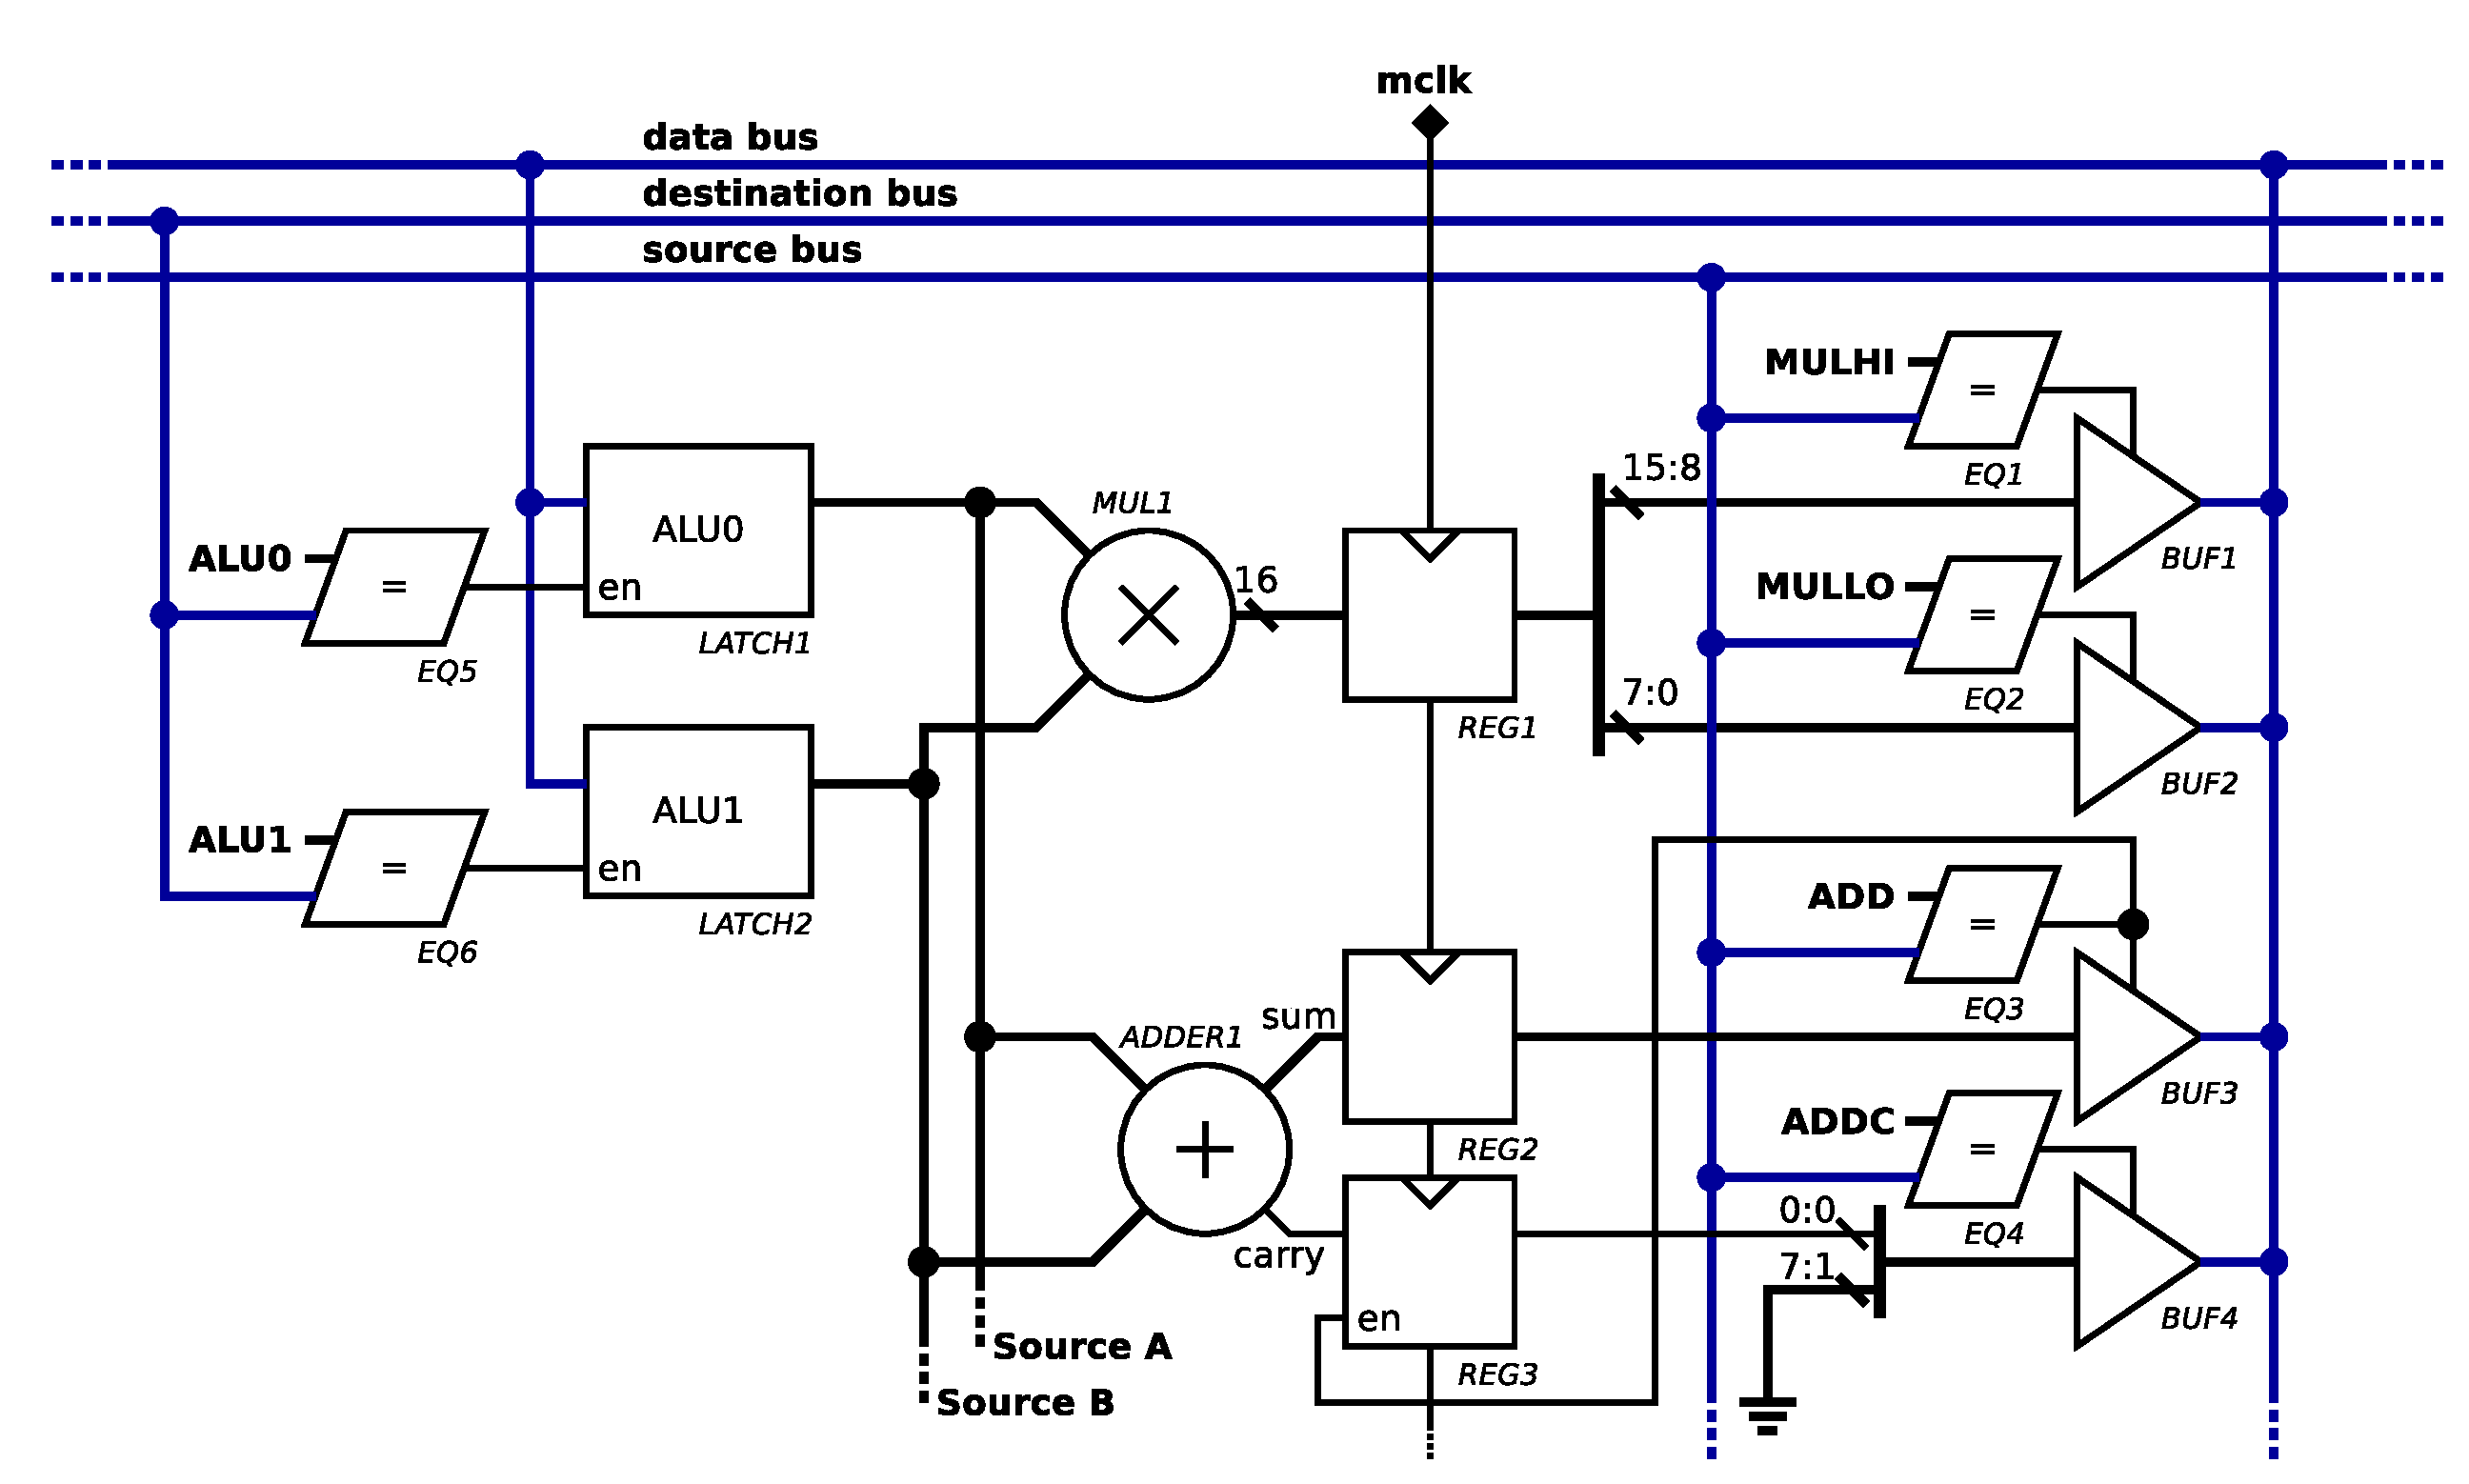
\includegraphics[scale=0.35]{../resources/oisc_alu.eps}
\caption{Digital diagram of OISC partial ALU logic}
\label{fig:oisc_alu}
\end{figure*}

This section will discuss ALU implementations of both processors. For fair comparison between OISC and RISC, ALU in both system will have the same capabilities described in table \ref{tab:alu_set}.

\begin{blockpage}
	\arrayrulecolor{black}
	\begin{tabular}{| c | p{0.75\linewidth} |} \hline 
		\rowcolor[rgb]{0.82,0.82,0.82}
		Name & Description \\\hline
		\arrayrulecolor[rgb]{0.82,0.82,0.82}
		ADD & Arithmetic addition (inc. carry) \\\hline
		SUB & Arithmetic subtraction (inc. carry) \\\hline
		AND & Bitwise AND \\\hline
		OR  & Bitwise OR \\\hline
		XOR & Bitwise XOR \\\hline
		SLL & Shift left logical \\\hline
		SRL & Shift right logical \\\hline
		ROL & Shifted carry from previous SLL \\\hline
		ROR & Shifted carry from previous SRL \\\hline
		MUL & Arithmetic multiplication \\\hline
		DIV & Arithmetic division \\\hline
		MOD & Arithmetic modulo \\
		\arrayrulecolor[rgb]{0,0,0}\hline
	\end{tabular}
	\captionof{table}{\textit{Supported ALU commands for both processors}}
	\label{tab:alu_set}
\end{blockpage}

\subsubsection{OISC ALU}
Due to the structure of OISC processor, ALU source A and B are two latches that are written into when \texttt{ALU0} or \texttt{ALU1} destination address is present. ALU sources are connected with every ALU operator and performed in single clock cycle. This value is stored in register so that it would immediately available in a next clock cycle as a source data. Figure \ref{fig:oisc_alu} represents logic diagram of ALU with only addition and multiplication operators present. Note that output of \textit{EQ3} is connected to enable of \textit{REG3}, enabling output of carry to be only read after \texttt{ADD} source is requested. This previous source memory is also used for \texttt{SUB}, \texttt{ROL} and \texttt{ROR} operations. This allows processor to perform other operations such as store or load values, before accessing carry bit, or carried byte for \texttt{ROL} and \texttt{ROR} operations.

\subsubsection{RISC ALU}
RISC processor has very similar structure to OISC with two exceptions. Inputs to ALU comes from logic router that decided how to route data in datapath. Output buffers are replaced by one multiplexer that selects single output from all ALU operations. Another point is that RISC ALU output is 16bit, higher byte saved in "ALU high byte register" for \texttt{MUL}, \texttt{MOD}, \texttt{ROL} and \texttt{ROR} operations. This register is accessible with \texttt{GETAH} instruction.

\subsection{Program Memory}\label{subsec:memory}
This section describes how instruction memory (ROM) is implemented for both processors.

\begin{figure*}[b]
	\centering
	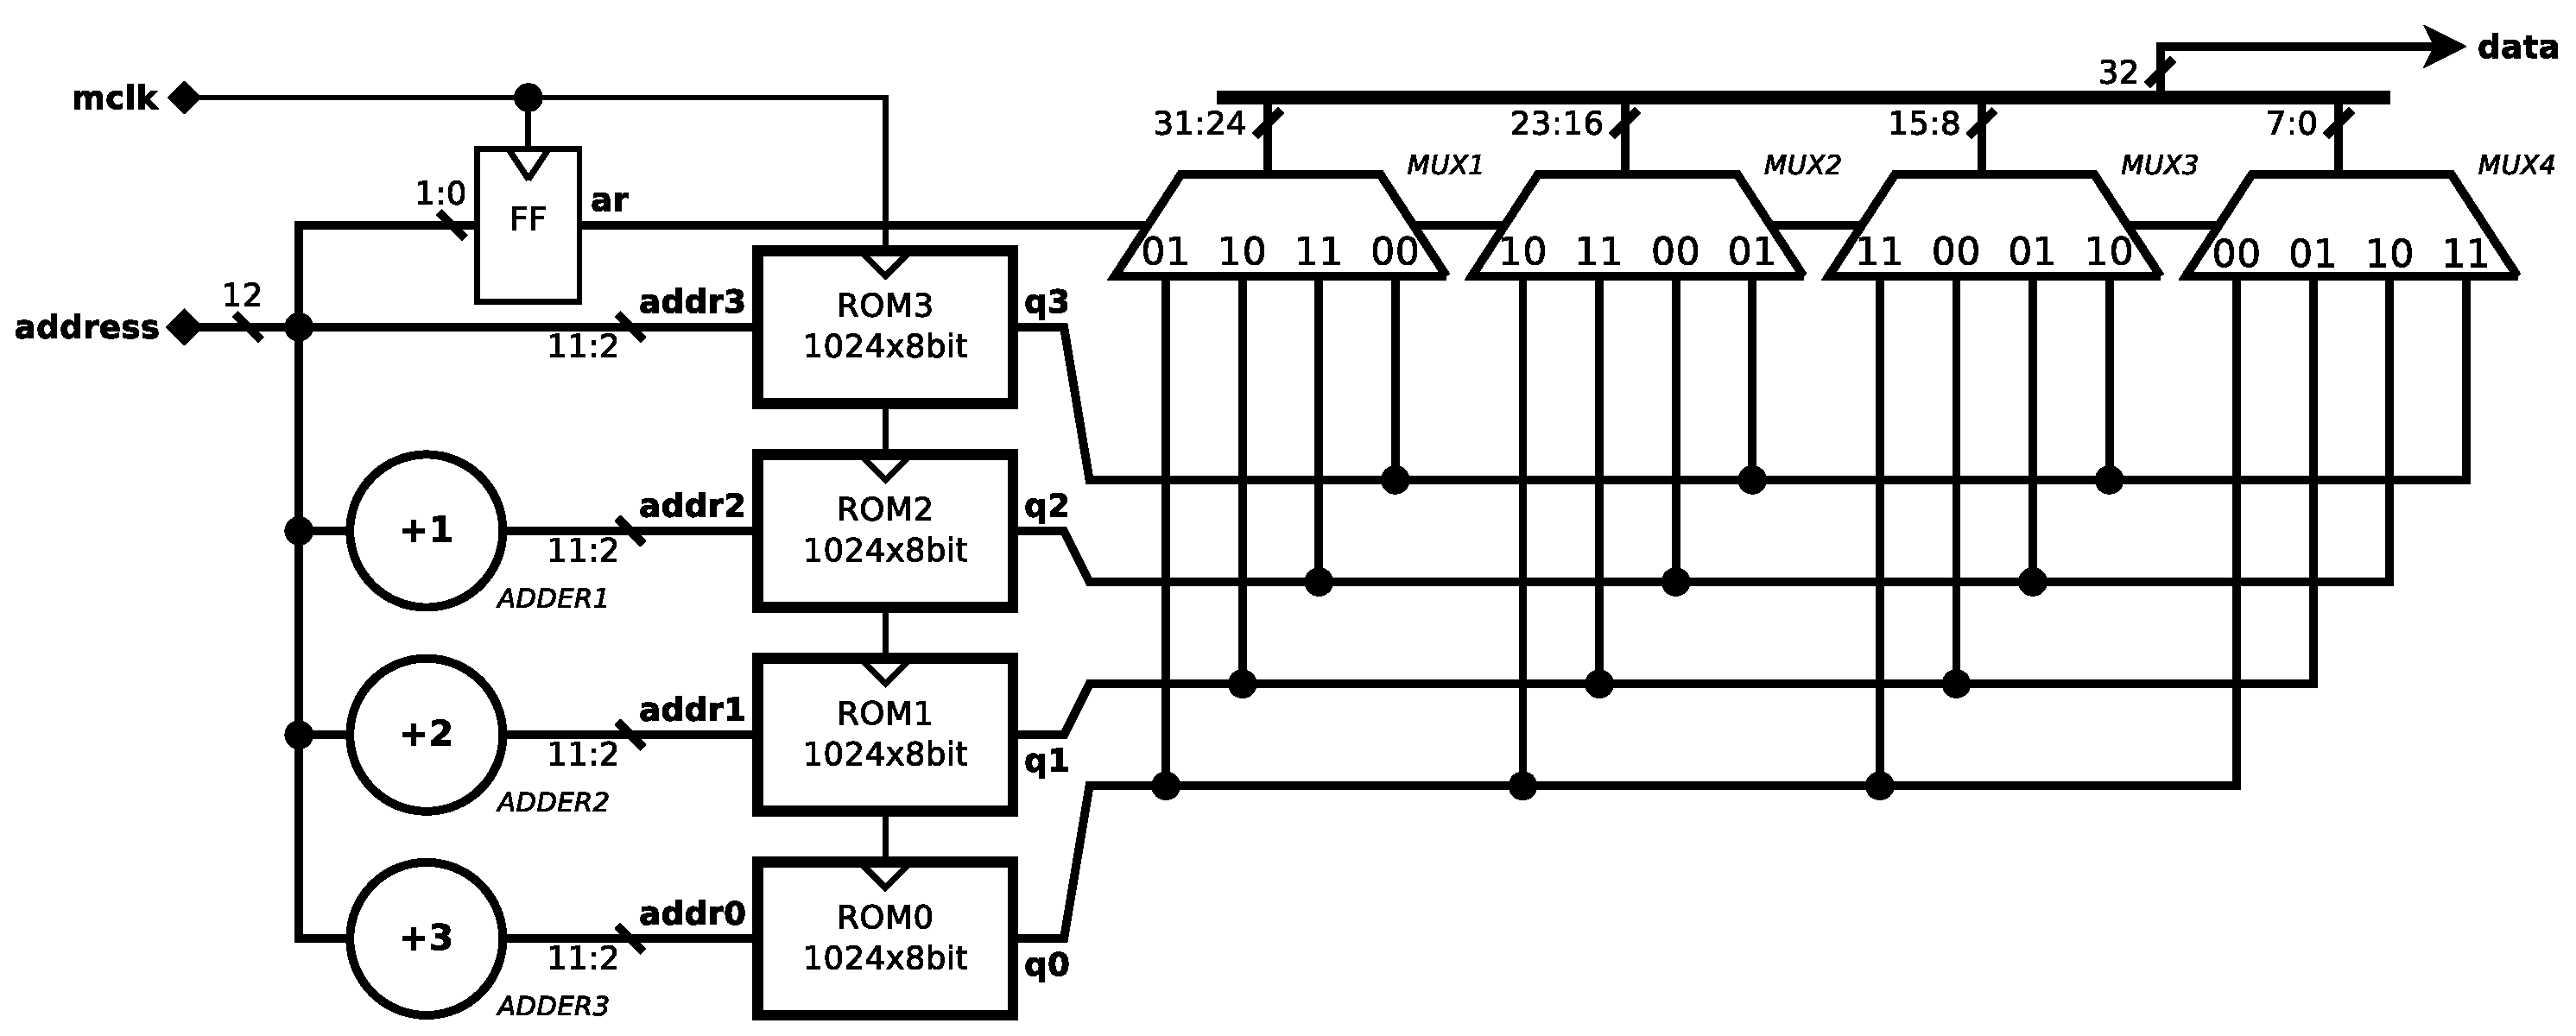
\includegraphics[width=\linewidth]{../resources/risc_mem.eps}
	\caption{Digital diagram of RISC sliced ROM memory logic}
	\label{fig:risc_mem}
\end{figure*}

\subsubsection{RISC Program Memory}
In order to allow dynamic instruction size from one to four bytes a special memory arrangement is made. A system was required to access word (8bits) from memory and next three words. To achieve this four ROM blocks been utilised, each containing one fourth of sliced original data. Input address is offset by adders \textit{ADDER1-3} and further divided by four by removing two least significant bits at \textbf{addr0-3}. 
Before concatenating output of each ROM block into final four bytes, ROM outputs \textbf{q0-3} are rearranged depending on \textbf{ar} signal. Note that \textit{MUX1-4} each input is different, this may be better visualised with Verilog code in listing \ref{code:rom_switch}.



\begin{blockpage}
\begin{lstlisting}[frame=single, language=Verilog, caption={RISC sliced ROM memory multiplexer arrangement Verilog code}, emph={ar, data}, label=code:rom_switch]
case(ar)
  2'b00: data={q3,q2,q1,q0};
  2'b01: data={q0,q3,q2,q1};
  2'b10: data={q1,q0,q3,q2};
  2'b11: data={q2,q1,q0,q3};
endcase
\end{lstlisting}
\end{blockpage}

\subsubsection{OISC Program Memory}\label{subsec:oisc_mem}
OISC instructions are fixed 13 bits, which causes different problems to RISC sliced memory - non-standard memory word size. To implement ROM in FPGA, Altera Cyclone IV M9K memory configurable blocks were used. Each blocks as 9kB of memory each allowing 1024x9bit configuration. Combining three of such blocks together yields 27bits if readable data in single clock cycle. To store instruction code to such configuration, pairs of instruction machine code sliced into three parts plus one bit for parity check, see figure \ref{fig:oisc_memory_slice}. Circuit extracting each instruction is fairly simple, shown in figure \ref{fig:oisc_mem}.

\begin{figure*}[t]
\begin{gather*}
\overunderbraces{&\br{1}{ROM0}&\br{2}{ROM1}&\br{2}{ROM2}}%
{&
\colorbox{c1}{\scalebox{0.75}{00}}\,
\colorbox{c1}{\scalebox{0.75}{01}}\,
\colorbox{c1}{\scalebox{0.75}{02}}\,
\colorbox{c1}{\scalebox{0.75}{03}}\,
\colorbox{c1}{\scalebox{0.75}{04}}\,
\colorbox{c1}{\scalebox{0.75}{05}}\,
\colorbox{c1}{\scalebox{0.75}{06}}\,
\colorbox{c1}{\scalebox{0.75}{07}}\,
\colorbox{c1}{\scalebox{0.75}{08}}\,&
\colorbox{c1}{\scalebox{0.75}{09}}\,
\colorbox{c1}{\scalebox{0.75}{10}}\,
\colorbox{c1}{\scalebox{0.75}{11}}\,
\colorbox{c1}{\scalebox{0.75}{12}}\,&
\colorbox{c2}{\scalebox{0.75}{13}}\,
\colorbox{c2}{\scalebox{0.75}{14}}\,
\colorbox{c2}{\scalebox{0.75}{15}}\,
\colorbox{c2}{\scalebox{0.75}{16}}\,
\colorbox{c2}{\scalebox{0.75}{17}}\,&
\colorbox{c2}{\scalebox{0.75}{18}}\,
\colorbox{c2}{\scalebox{0.75}{19}}\,
\colorbox{c2}{\scalebox{0.75}{20}}\,
\colorbox{c2}{\scalebox{0.75}{21}}\,
\colorbox{c2}{\scalebox{0.75}{22}}\,
\colorbox{c2}{\scalebox{0.75}{23}}\,
\colorbox{c2}{\scalebox{0.75}{24}}\,
\colorbox{c2}{\scalebox{0.75}{25}}\,&
\colorbox{c3}{\scalebox{0.75}{26}}\,&
}%
{&\br{2}{InstrA}&\br{2}{InstrB}&\br{1}{parity}}
\end{gather*}
\caption{OISC three memory words composition. Number inside box represents bit index.}
\label{fig:oisc_memory_slice}
\end{figure*}

\begin{figure*}[t]
	\centering
	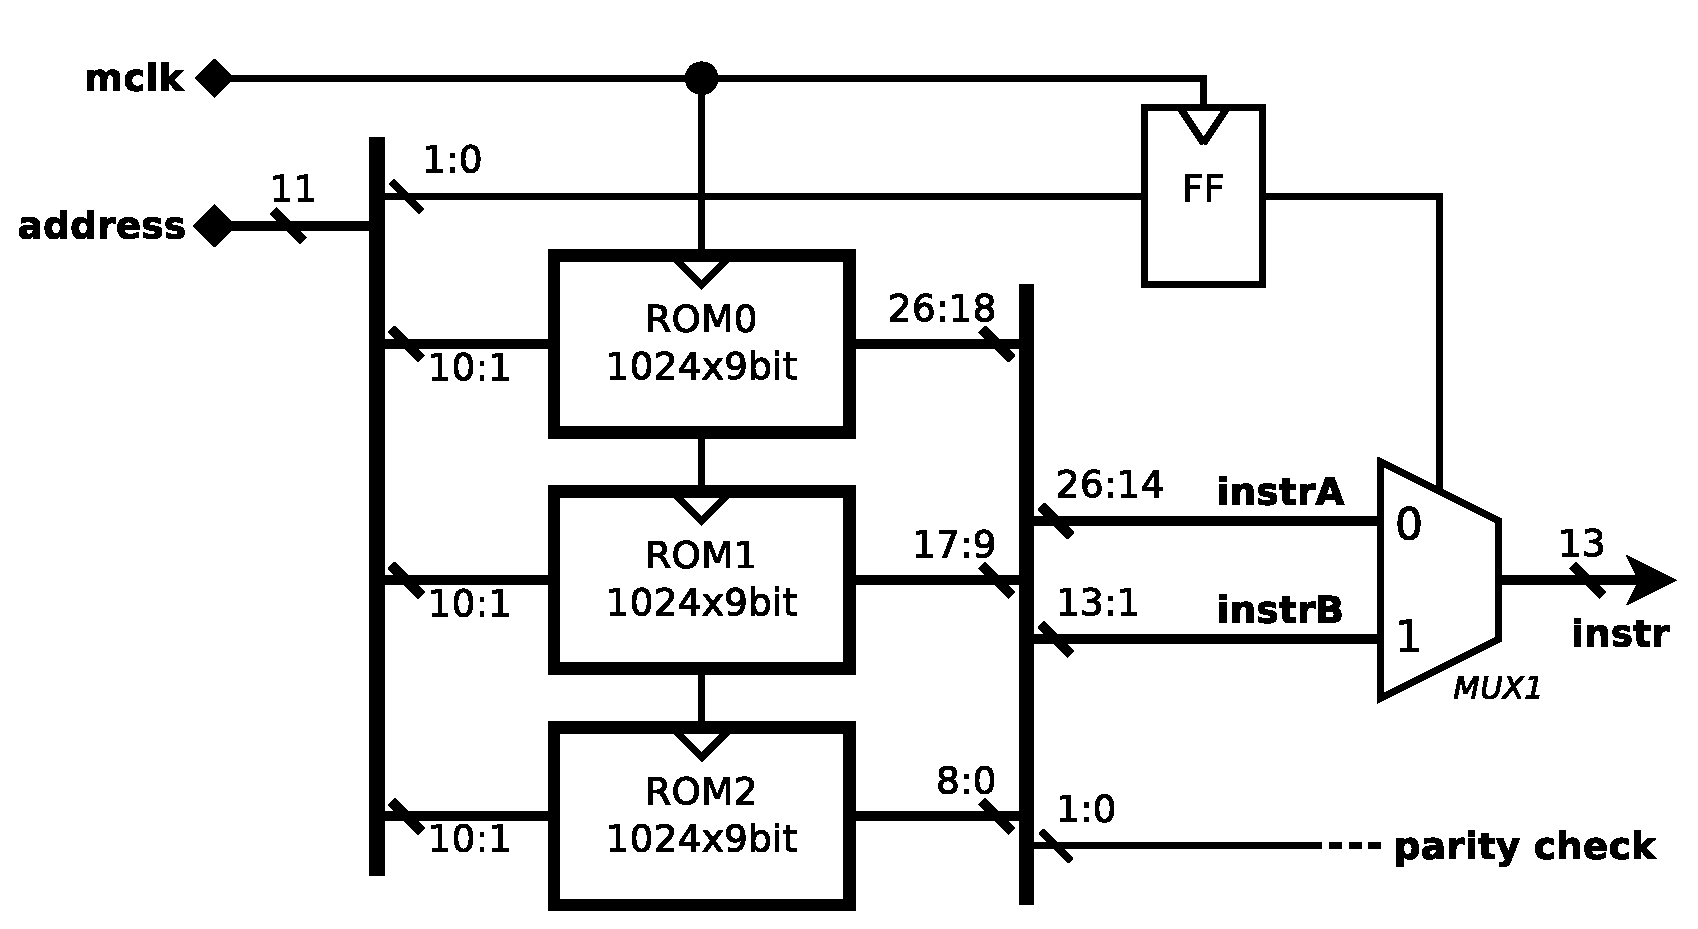
\includegraphics[scale=0.4]{../resources/oisc_mem.eps}
	\caption{Digital diagram of OISC instruction ROM logic}
	\label{fig:oisc_mem}
\end{figure*}

\subsection{Instruction decoding}\label{subsec:imm_values}
This section describes RISC and OISC differences between instruction decoding and immediate value handling.
\subsubsection{RISC IMO} \label{subsec:imo}
Already described in previous section \ref{subsec:memory}, instruction from memory comes as 4 bytes. Least significant byte is sent to control block, other three bytes are sent to immediate override block (IMO) shown in figure \ref{fig:risc_imo}. These three bytes are labelled as \textbf{immr}. 

\begin{figure*}
	\centering
	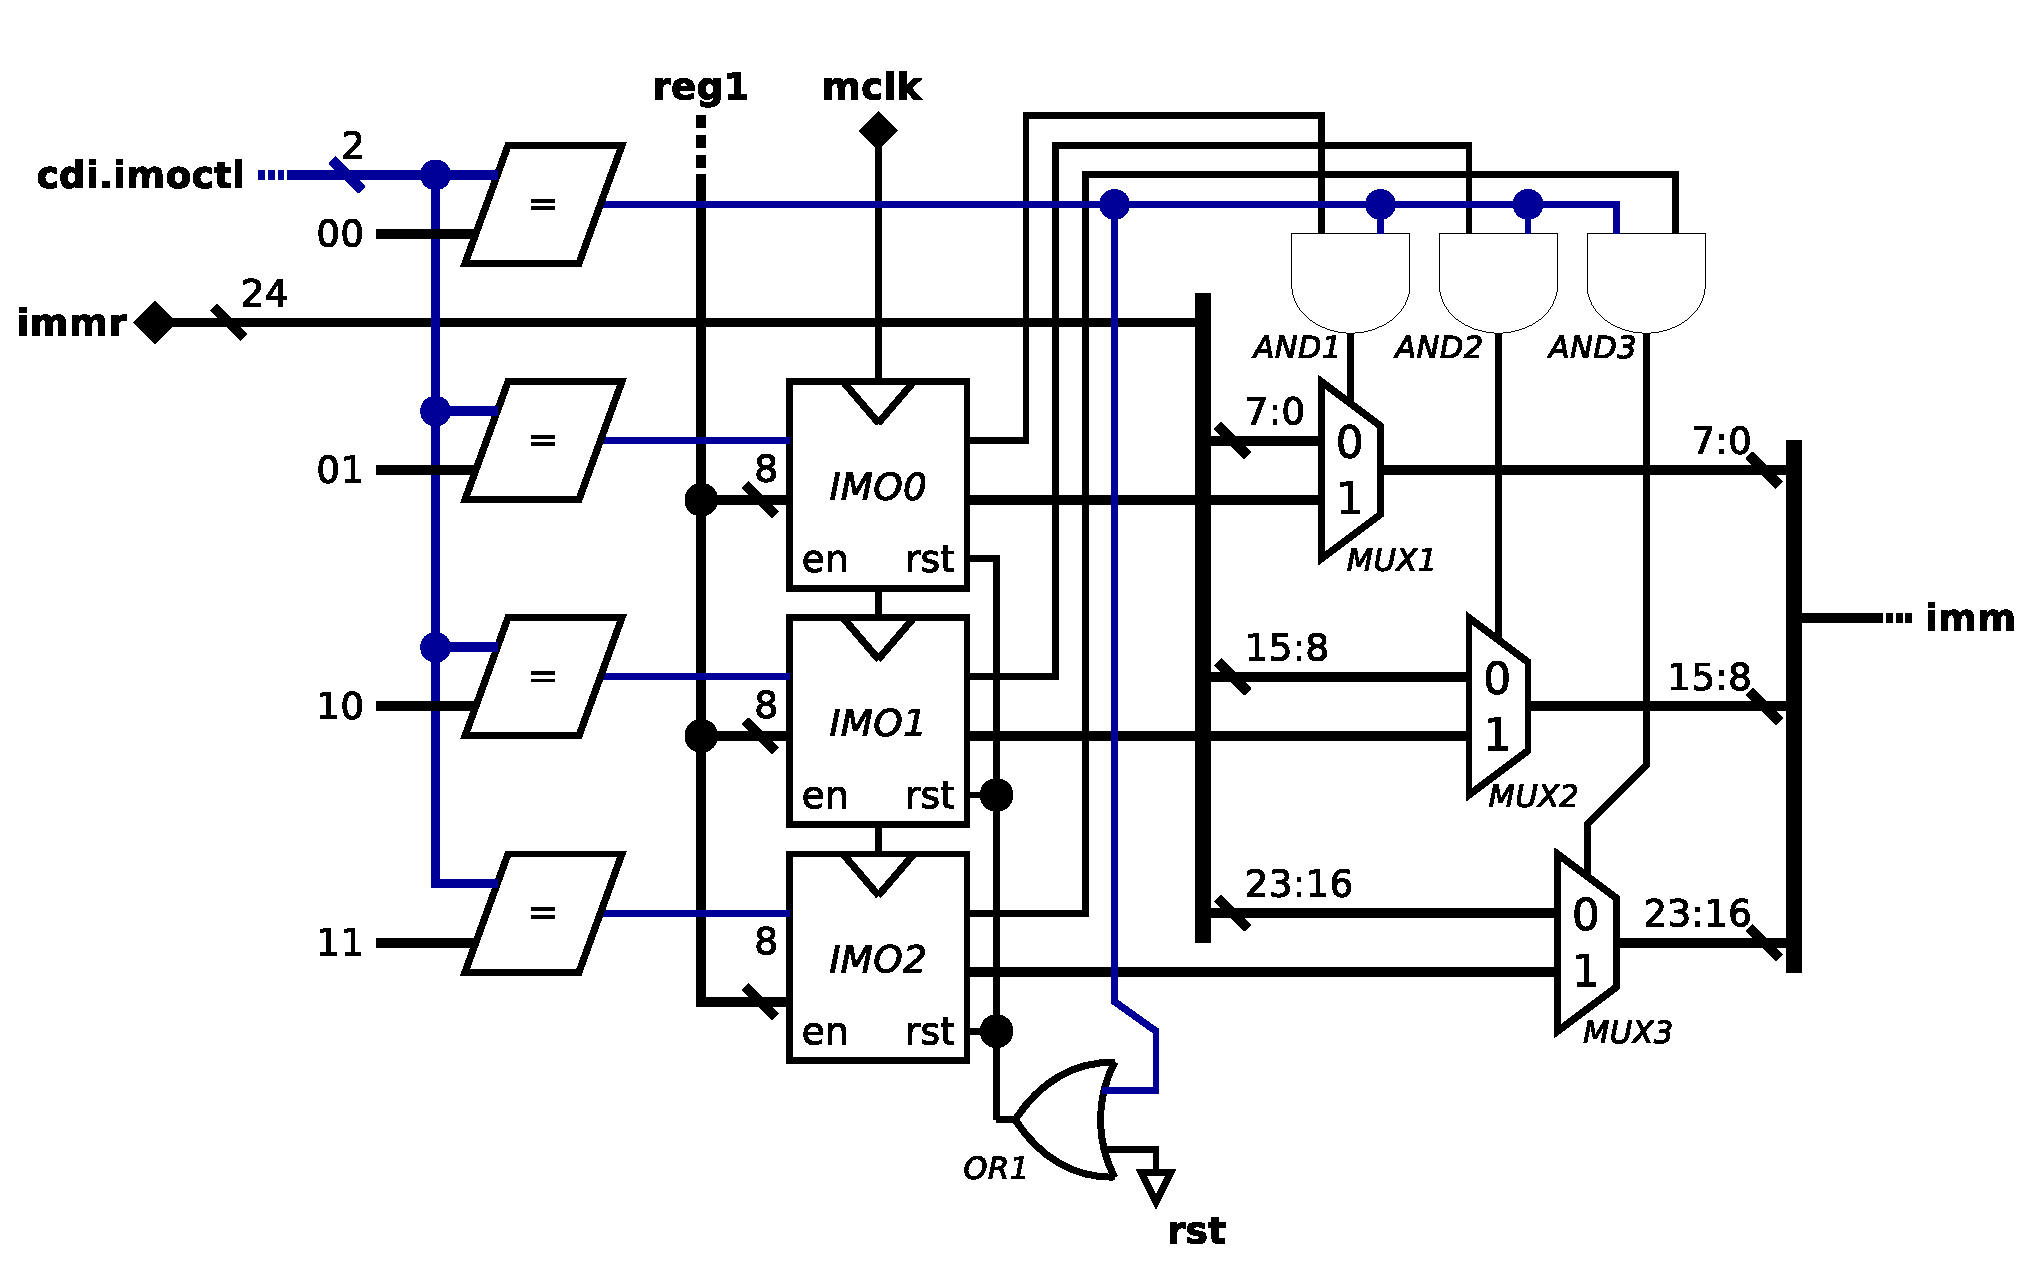
\includegraphics[scale=0.4]{../resources/risc_imo.eps}
	\caption{Digital diagram of RISC immediate override system}
	\label{fig:risc_imo}
\end{figure*}


IMO block is a solution to change immediate value which enabled dynamically calculated memory pointers, branches dependant on register value or any other function that needs instruction immediate value been replaced by calculated register value. IMO is controlled by control block and \textbf{cdi.imoctl} signal, which is changed by \texttt{CI0}, \texttt{CI1} and \texttt{CI2} instructions. When signal is \texttt{0h}, this block is transparent connecting \textbf{immr} directly to \textbf{imm}. When any of \texttt{CI} instructions executed, one of IMO register is overridden by \textit{reg1} value from register file. In order to override two or three bytes of immediate, \texttt{CI} instructions need to be executed in order. Only for one next instruction after last \texttt{CI} will have immediate bytes changed depending on what are values in \textit{IMO} registers.
\\This circuit has two disadvantages: 
\begin{enumerate}
	\item Overriding immediate bytes takes one or more clock cycles,
	\item At override, \textbf{immr} bytes are ignored therefore they are wasting instruction memory space.
\end{enumerate}
Second point can be resolved by designing a circuit that would subtract the amount of overridden IMO bytes from \textit{pc\_off} signal (program counter offset that is dependant on i-size value) at the program counter, thus effectively saving instruction memory space. This solution however would introduce a complication with the assembler as additional checks would need to be done during compiling to check if IMO instruction are used.

\subsubsection{OISC Instruction decoding}
OISC immediate value is set in instruction decoder shown in figure \ref{fig:oisc_decoder}. Decoder operation is simple - instruction machine code is split into three parts as described in \ref{fig:oisc_machinecode}. If instruction source address is \texttt{00h}, connect data bus with constant 0 via \textit{MUX2}. If immediate bit is 1, set source address to \texttt{00h} (to make sure no other buffer source connects to data bus), and connect instruction source address (immediate value) to databus via \textit{MUX2} and \textit{BUF1}. 

\begin{figure*}
	\centering
	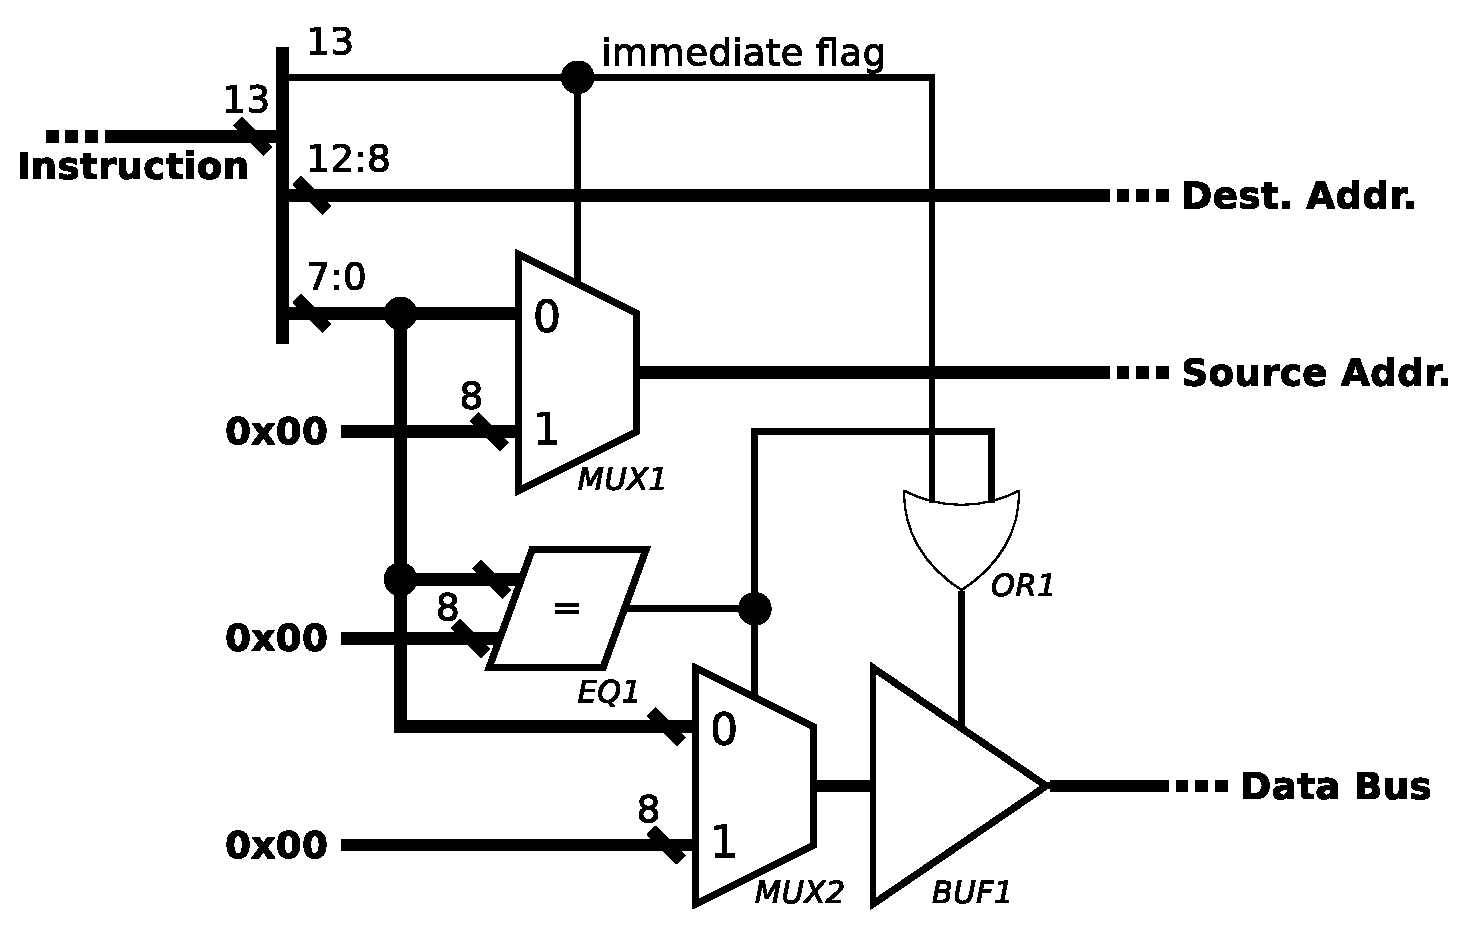
\includegraphics[scale=0.4]{../resources/oisc_decoder.eps}
	\caption{Digital diagram of OISC instruction decoder}
	\label{fig:oisc_decoder}
\end{figure*}

\subsection{Assembly}\label{subsec:assembly}

There are two steps between assembly code and its execution on a processor. First it needs to be converted to binary machine code. Secondly, binary data needs to be sliced to different parts described in section \ref{subsec:memory}. These slices also need to be converted into appropriate formats, as simulation, HDL synthesis and flashing memory directly to FPGA memory, all use different formats.


A universal assembler was implemented with python for both processors. Flowchart in figure \ref{fig:assembler} represents general structure of assembler process. It splits assembly file into three parts - sections, definitions and macros. Definitions are keywords mapped to values which are saved in global label dictionary. Macros are a chunk of assembly code and is used as templates. 

There are only two sections implemented in assembler - \texttt{.text} and \texttt{.data}. Section \texttt{.text} contains all machine instructions which will be stored in program ROM memory. Section \texttt{.data} is used for global and static data, and it will be written into RAM memory. This section contains values such as strings and structures uninitialised data as labels which data is RAM memory location. 

Section \texttt{.text} is processed line by line. Each has label, instruction name and instruction arguments. Label however is optional, if line contains it, label is saved to global label dictionary with program address. If line instruction name is a macro, line is replaces by macro and instruction arguments are used as macro arguments. Otherwise instruction name is decoded and stored in instruction list with original arguments.

After all instruction lines are completed, each stored instruction arguments are processed, labels are replaced with binary values, any other processing is done such as addition by constant, byte selection, etc. Completed list is then saved as raw binary. Similarly, \texttt{.data} section labels also replaced and it is saved as binary data.

\begin{colfigure}
	\centering
	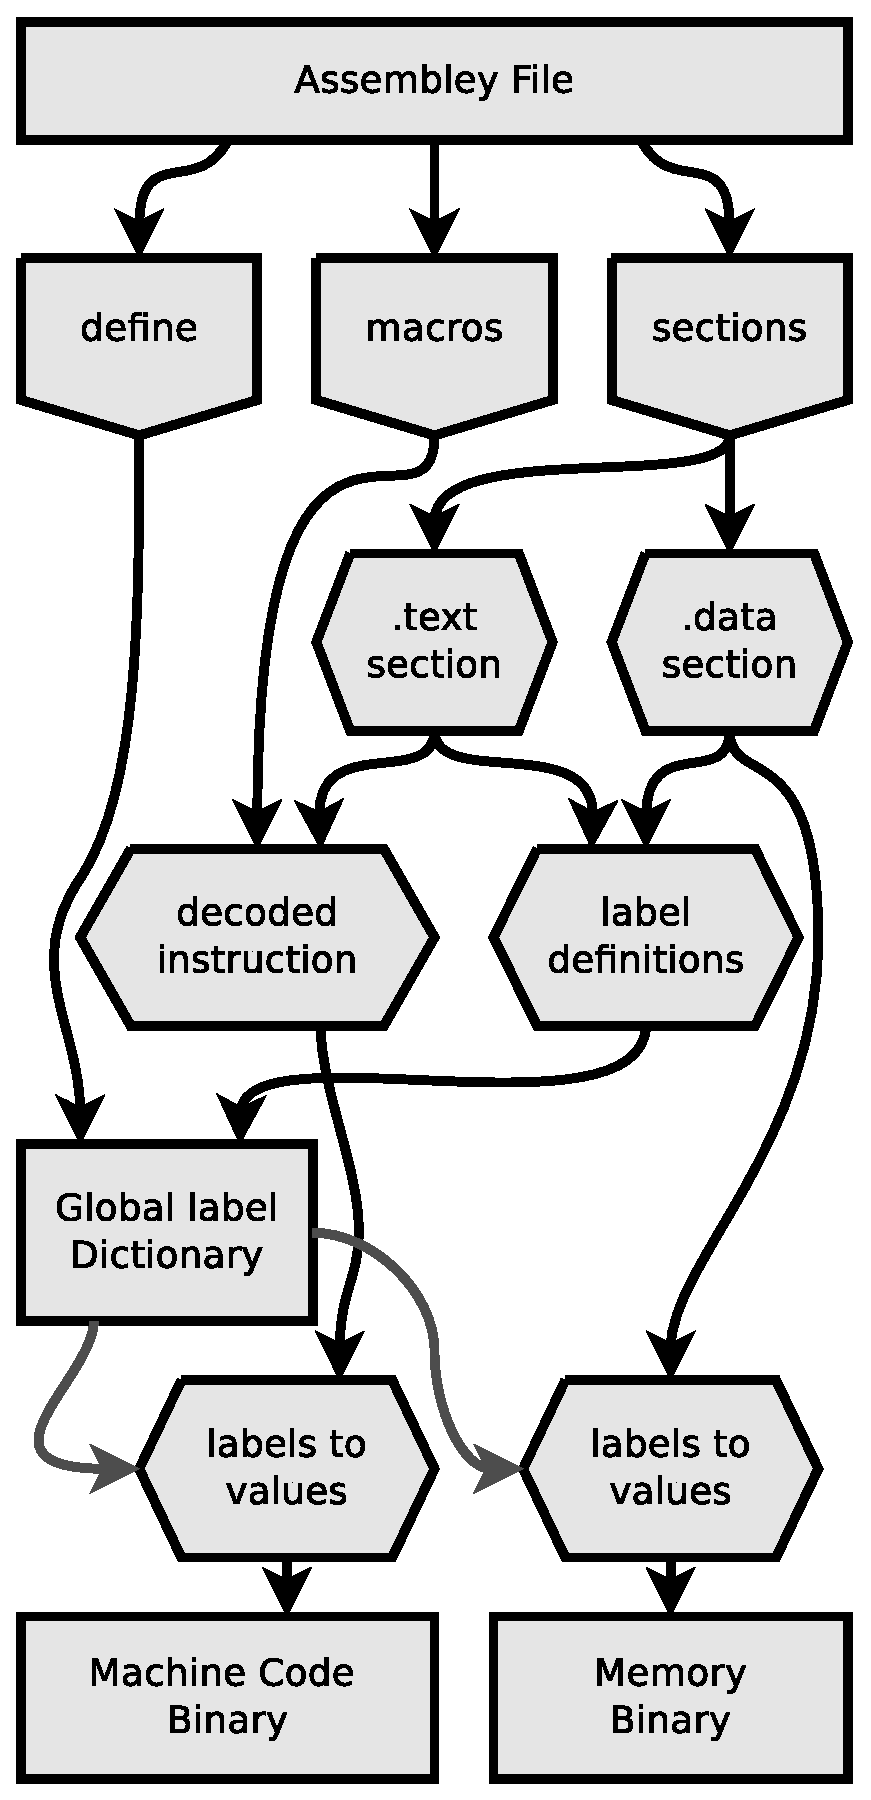
\includegraphics[scale=0.4]{../resources/assembler.eps}
	\captionof{figure}{Flow chart of assember converting assembly code into machine code and memory binary.}
	\label{fig:assembler}
\end{colfigure}

\subsection{System setup}\label{subsec:setup}
This section will describe how system is setup.

Processors are implemented on Terasic DE0-Nano board that use Altera Cyclone IV, EP4CE22P17C6 FPGA, which is manufactured using $60nm$ fabrication technology.
FPGA has embedded memory structure consisting of columns of M9K memory blocks mentioned in Subsection \ref{subsec:oisc_mem}. These memory structures were used to implement processors RAM and ROM memories. Board also has 32MB SDRAM chip, which initially was intended to be used. This set design criteria to have 24bit address space. However, M9K memory was used instead for simplicity. 

FPGA has embedded phase-locked loop (PLL) stucture that is used to change 50MHz input that is generated by on-board crystal to other frequencies. 

DE0-Nano board as integrated JTAG port that is used to upload synthesised code and additional debugging tools. Quartus has "Signal Tap Logic Analyzer" tools that allow setup probes and sources within FPGA logic and control them via JTAG. "In-System Memory Content Editor" tool allows read and modify M9K memory which enabled quick machine code uploading to FPGA without need to resynthesise HDL code. This also allow reading RAM content to debug program. 

All Quartus functions can be implemented via TCL script. This allowed constructing Makefile to allow quick build functions. Quatus signal and memory tool functions were used to write a small program with Python and Curses library to read and change internal processor state which allowed easy debugging while writing programs. 



	\vfill\pagebreak
	\section{Results and Analysis}\label{sec:results}
	% !TeX root = index.tex
\iffalse
This chapter looks specifically at your results.
* You measured some samples. 
What values did you measure? 
Present them in a table or graph? 
How did you test whether they were good measurements? 
Were you looking to improve something? 
Are your new samples better than the old ones?

* You built a device; 
what tests did you run to make sure that it is running correctly?

* You calculated something or developed a new theory about something. 
How do you know how well it predicts? 
What tests did you run? 
What comparisons with the literature did you make?
* You coded or simulated something. 
What tests did you run to be sure it was working correctly? 

Describe what you want the reader to notice in the results. 
Give the facts, then give your analysis of the facts.
Present your graphs, figures, tables, photos, and equations needed to show what you accomplished.
Label everything clearly, using the recommendations given below in “Things to Look For”
\fi

\subsection{FPGA logic component composition}
This subsection looks at specific test and its results which finds how much FPGA logic components each processor takes and what is composition of each part.

The test was performed with Quartus synthesis tool by recording flow summary report data. This report includes synthesised design metrics including total logic elements, registers, memory bits and other FPGA resources. In this test, only parameters that were recorded are logic elements and registers. Number of resources was found by synthesising full processor, then commenting relevant parts of code, re-synthesising and viewing changes in the report. Such method may not be the most accurate, because during HDL synthesis, circuit is optimised and unused connections removed. This means that more of the logic than commented may be not synthesised. 

There are four parts of each processor that will be tested: 
\begin{enumerate}
	\item \textbf{Common} - processor auxiliary logic that is used by both processors. It includes the communication block with UART, RAM and PLL (Phase-Locked Loop, for master clock generation). 
	\item \textbf{ALU} - as described in section \ref{subsec:alu}, both processors have slightly different implementation of ALU.
	\item \textbf{Memory} - the processors memory management, including stack.
	\item \textbf{Other} - reminding processor logic that was not analysed.
\end{enumerate}

\begin{colfigure}
	\centering
	\includegraphics[width=\linewidth]{../tests/fpga_comp.eps}
	\captionof{figure}{Bar graph of FPGA logic components taken by each processor.}
	\label{fig:fpga_comp}
\end{colfigure}

The test results are shown in figures \ref{fig:fpga_comp} and \ref{fig:fpga_reg_comp}. The common logic uses 293 logic elements and 170 registers. OISC uses 1705 logic elements, while RISC uses 3218. Excluding common logic, OISC takes 48.3\% of RISC's logic elements.


\begin{colfigure}
	\centering
	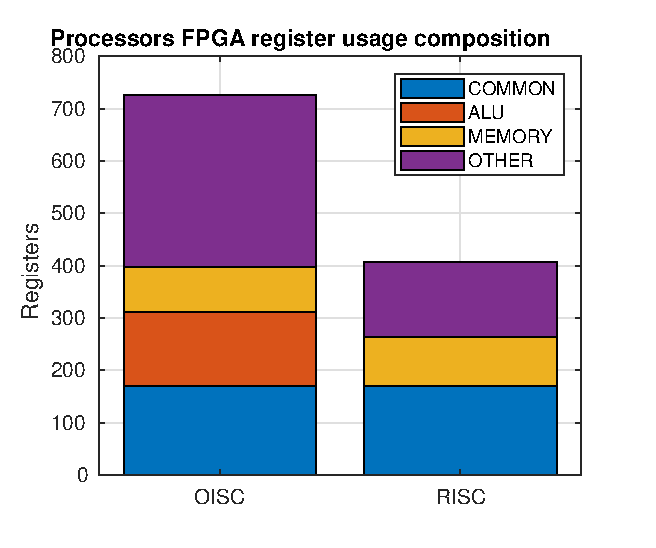
\includegraphics[width=\linewidth]{../tests/fpga_reg_comp.eps}
	\captionof{figure}{Bar graph of FPGA register resources taken by each processor.}
	\label{fig:fpga_reg_comp}
\end{colfigure}

OISC uses 726 logic elements, while RISC uses only 407. Excluding common logic, OISC uses 78.4\% more registers than RISC.

Looking at the composition, OISC ALU takes 30.2\% more logic gates. Figure \ref{fig:fpga_reg_comp} shows high number of OISC ALU registers. This concludes that higher resource usage in OISC ALU code must be source and destination logic.

Memory logic element composition of OISC is only 34.4\% of RISC's and 7\% lower for register resources, comparing to RISC. This indicates that by removing memory logic for RISC, synthesis tool may removed also other parts of processor, possibly part of control block because it mostly contains combinational logic.

Other logic includes instruction decoding with ROM, register file, program counter. RISC exclusively has control block. Note that OISC uses only three ROM memory blocks whereas RISC uses four as explained in section \ref{subsec:memory}, however this should make a minimal difference as M9K memory blocks are not included in FPGA logic element or register count. Comparing both processors, OISC has only 37\% of other logic components to RISC, however it has 2.28 times more registers. This shows a logic component - register trade-off. OISC source and destination logic requires more registers, whereas RISC uses combination logic in control block in order to control the same data in datapath. 

Much higher logic components in RISC can be also explained more complicated register file, ROM memory logic and program counter. All of these components has some additional logic for timing correction or other extra functionality required by these block integration into a datapath.

\subsection{Power analysis}

Power analysis was performed to analyse power consumption of both processors.
This has been accomplished by connecting FPGA board to a laboratory power supply with 4V to an external power input. A shunt resistor with impedance of 1.020$\Omega$ was connected in series to calculate current. Supply voltage and voltage across shut resistor were measured using an oscilloscope with a data sampling feature. Three tests have been performed with different processor configurations. Between each test a period of about 5 minutes was given for FPGA to reach steady state. 


\begin{colfigure}
	\centering
	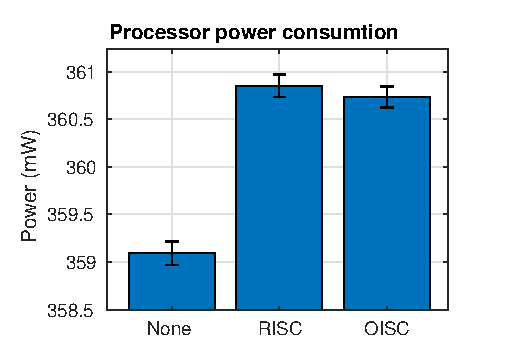
\includegraphics[width=\linewidth]{../tests/power.eps}
	\captionof{figure}{Measured power of processors when implemented on FPGA, running 16bit multiplication function in loop. None indicates auxiliary-only power.}
	\label{fig:power}
\end{colfigure}

Figure \ref{fig:power} represents power results. First configuration is "None" or auxiliary-only power, which includes whole FPGA board, voltage regulators, and synthesised logic on FPGA required to support a processor (such as PLL, UART, Input/Output control, RAM). RISC and OISC bars in the graph indicate processor implementations on FPGA, each running multiplication program in a loop. These values also include auxiliary power plus processor power, which means that the processor itself takes relatively small amount comparing to auxiliary power, about 0.5\%. Result shows that OISC require 0.4\%, which including noise is almost insignificant result.

During this test clock frequency of 1MHz was used. Due to equipment unavailability, any further tests were not carried out to investigate power consumption at different frequencies. Due to constant noise, running at higher frequency may result in significant difference between processors.

\subsubsection{Activity Factor}\label{subsec:activity_factor}
An activity factor could be also found using Equation \ref{eq:activity_factor} where $P$ is power, $C_{total}$ is total gate capacitance and $V_{DD}$ is voltage supplied to the transistors.
\begin{align}\label{eq:activity_factor}
\alpha = \frac{P}{C_{total}\cdot f \cdot V_{DD}^2}
\end{align}
As $C_{total}$ and $V_{DD}$ are constants, measuring power at different frequencies allows finding activity factor. This value could be used to compare how much of a processor circuit is active. Further design improvements could be used to optimise power \autocite{8682289,7363689,1207041,6972455}.


\subsection{Benchmark Programs}
A number of and programs have been written to test both processors. These involve simple functions that could be commonly used in a 8bit processors:

\begin{description}
	\item[$\bullet$ Printing:] Sends data to UART. It includes waiting until UART is available for transmission. 
	\item[$\bullet$ Printing unsinged integer:] Uses binary-coded decimal algorithm to convert 8 or 16bit binary value to decimal value and print it. 
	\item[$\bullet$ 16bit multiplication:] Uses simple matrix multiplication. 
	\item[$\bullet$ 16bit division:] Uses Long division algorithm to divide two 16bit numbers, result including a reminder.
	\item[$\bullet$ 16bit modulo:] Uses "Russian Peasant Multiplication" algorithm to perform Modulo operation with two 16bit numbers.
	\item[$\bullet$ Prime number calculator:] Uses Sieve of Atkins algorithm \autocite{morain_1989} to calculate primer number, operates on 16bit numbers and utilise 16bit multiplication and modulo functions. 
\end{description}


\subsubsection{Instruction composition}\label{subsec:instr_comp}

This test is performed to investigate instruction composition of each function to see how similar it is between RISC and OISC processors. 
\begin{description}
	\item[$\bullet$ MOVE] - All instructions that move data around internal processor registers.
	\item[$\bullet$ ALU] - Instructions that are used to perform ALU operation.
	\item[$\bullet$ MEMORY] - Instructions that are required to send/retrieve data from system memory, except stack.
	\item[$\bullet$ STACK] - Instructions that push/pop data from memory stack.
	\item[$\bullet$ COM] - Instruction(s) that send/receive data from communication block.
	\item[$\bullet$ BRANCH] - Instructions that are used to make program branching.
	\item[$\bullet$ OTHER] - Any other instructions.
\end{description}

\begin{blockpage}
	\arrayrulecolor{black}
	\begin{tabular}{| c | p{0.65\linewidth} |} \hline 
		\rowcolor[rgb]{0.82,0.82,0.82}
		Name & Instructions \\\hline
		MOVE & \texttt{MOVE, CPY0, CPY1, CPY2, CPY3, CI0, CI1, CI2} \\\hline
		ALU & \texttt{%
			ADD, ADDI,
			SUB, SUBI,
			AND, ANDI,
			OR, ORI,
			XOR, XORI,
			DIV, MUL,
			ADDC, SUBC,
			INC, DEC,
			SLL, SRL, 
			SRA, GETAH
		} \\\hline
		MEMORY & \texttt{LWLO, LWHI, SWLO, SWHI} \\\hline
		STACK  & \texttt{PUSH, POP} \\\hline
		COM & \texttt{COM} \\\hline
		BRANCH & \texttt{BEQ, BGT, BGE, BZ, JUMP, CALL, RET} \\\hline
		\arrayrulecolor[rgb]{0,0,0}\hline
	\end{tabular}
	\captionof{table}{RISC processor instruction groups used in instruction composition test.}
	\label{tab:instr_groups_risc}
\end{blockpage}

\begin{blockpage}
	\arrayrulecolor{black}
	\begin{tabular}{| c | p{0.65\linewidth}|} \hline 
		\rowcolor[rgb]{0.82,0.82,0.82}
		Name & Destination \\\hline
		\arrayrulecolor[rgb]{0.82,0.82,0.82}
		MOVE & \texttt{REG0, REG1} \\\hline
		ALU & \texttt{ALU0, ALU1} \\\hline
		MEMORY & \texttt{MEM0, MEM1, MEM2, MEMLO, MEMHI} \\\hline
		STACK  & \texttt{STACK}\\\hline
		COM & \texttt{COMA, COMD}\\\hline
		BRANCH & \texttt{BR0, BR1, BRZ}\\\hline
		\arrayrulecolor[rgb]{0,0,0}\hline
	\end{tabular}
	\captionof{table}{OISC processor instruction desination groups used in instruction composition test}
	\label{tab:instr_groups_oisc_dst}
\end{blockpage}

\begin{blockpage}
	\arrayrulecolor{black}
	\begin{tabular}{| c | p{0.65\linewidth} |} \hline 
		\rowcolor[rgb]{0.82,0.82,0.82}
		Name & Instructions \\\hline	
		\arrayrulecolor[rgb]{0.82,0.82,0.82}	
		MOVE & \texttt{ALU0, ALU1, REG0, REG1, PC0, PC1, NULL, IMMEDIATE} \\\hline
		ALU & \texttt{ADD, ADDC, SUB, SUBC,
		AND, OR, XOR, SLL,
		SRL, EQ, GT, GE, NE,
		LT, LE, MULLO, MULHI, DIV, MOD,
		ADC, SBC, ROL, ROR} \\\hline
		MEMORY & \texttt{MEM0, MEM1, MEM2, MEMLO, MEMHI} \\\hline
		STACK  & \texttt{STACK} \\\hline
		COM & \texttt{COMA, COMD} \\\hline
		BRANCH & \texttt{BR0, BR1} \\\hline
		\arrayrulecolor[rgb]{0,0,0}\hline
	\end{tabular}
	\captionof{table}{OISC processor instruction source groups used in instruction composition test}
	\label{tab:instr_groups_oisc_src}
\end{blockpage}

Each function was executed on a simulated processor, program counter and instruction were recorded into file at every cycle. File recording was accomplished with SytemVerilog test bench. Start of a recording was triggered when program counter matched \texttt{.start} location and stopped when it matched \texttt{.done} location. Code shown in Listing \ref{code:asmtest} enabled both locations to be static and not depend on test function that was executed.

\begin{blockpage}
	\begin{lstlisting}[frame=single, caption={Assembly frame for executring tests}, emph={setup,start,done}, label={code:asmtest}]
setup:
  JUMP .start
.done:
  JUMP .done
.start:
  ; Setup values
  ; Call function
  JUMP .done
	\end{lstlisting}
\end{blockpage}

\begin{figure*}[t]
	\centering
	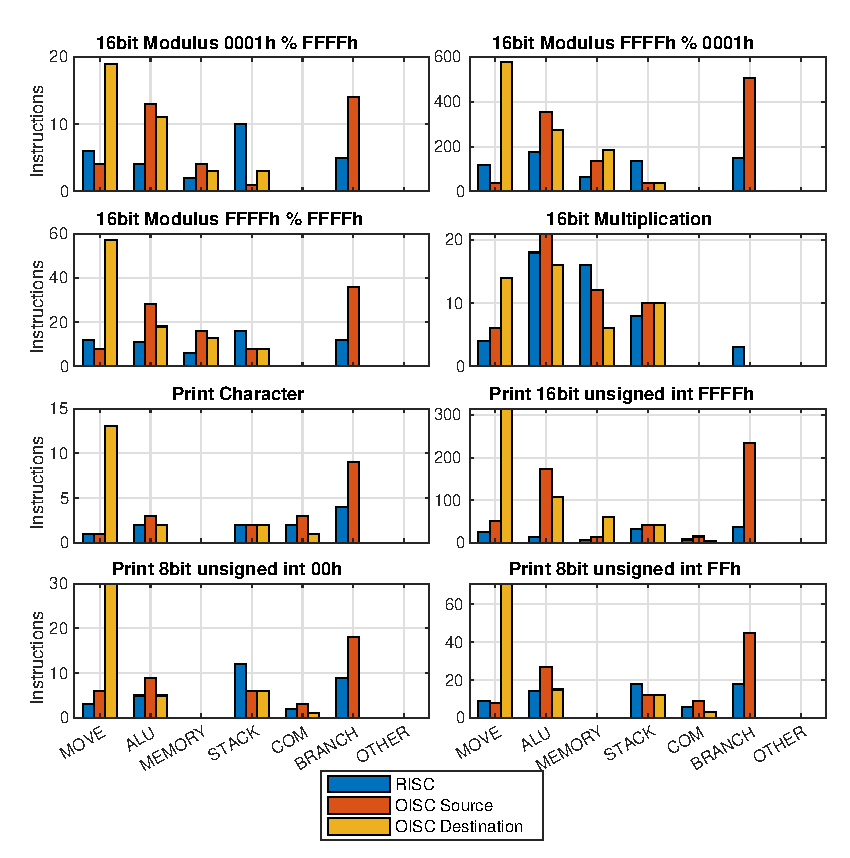
\includegraphics[width=\linewidth]{../tests/instr_comp.eps}
	\caption{Graph of instruction composition for every benchmark program.}
	\label{fig:instr_comp}
\end{figure*}


Each recorded file with function composition was then further analysed and each instruction was grouped. Recorded program counter was used to find effective program space. This has been achieved by calculating unique instances of program counter and summing up instruction size for each of them. In RISC, dynamic instruction size has been taken into account. 

From the results in Figure \ref{fig:instr_comp}, few key differences can be seen. Across every test, OISC has significantly more \textit{BRANCH} destination and \textit{MOVE} source groups. \textit{BRANCH} group can be explained by emulated \texttt{CALL}, \texttt{RET} and \texttt{JUMP} instruction explained in section \ref{subsec:oisc_pc}.
High number of \textit{MOVE} source group instructions may be explained by using the immediate values as a separate source, where RISC uses instructions that can integrate immediate as extra word, such as instruction \texttt{ADDI}. In most cases \textit{ALU} group instructions are also higher than for OISC comparing to RISC. This shows a lower OISC ALU efficiency, mostly due to a need to move data into the septate accumulators.

\subsubsection{Performance}
This subsection investigates time and clock cycles to run benchmark programs. The simulation was performed to find a number of cycles required to execute each function. Note that prime number calculator was not simulated due to too complex dynamic nature of program. 

Print 16bit decimal and modulo operation were executed with different input arguments. This allows to see the worst and the best case scenarios as algorithms length depend on inputs. This is not the case for 16bit multiplication as its implementation has no branching, therefore no execution time dependence on the inputs.

Results are shown in Figure \ref{fig:cycles}. In most of the cases, OISC requires around 55-67\% more instructions, with some exceptions.

\begin{colfigure}
	\centering
	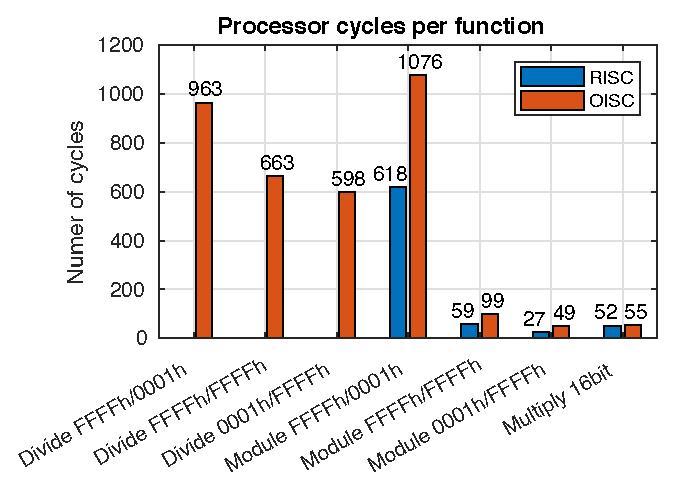
\includegraphics[width=\linewidth]{../tests/cycles.eps}
	\captionof{figure}{Simulated results of cycles that taken to perform function.}
	\label{fig:cycles}
\end{colfigure}

Another set of benchmarks have been performed and on both processors once they been implemented on the FPGA. Time taken for perform each set has been recorded. This has been done via UART connection, a single character was sent to indicate the start and the stop of a benchmark. In order to void a slight timing variation due low baud rate of UART or system kernel scheduler unpredictability to process UART input, each benchmark was performed with many iterations. Figure \ref{fig:timing} represents results.

\begin{colfigure}
	\centering
	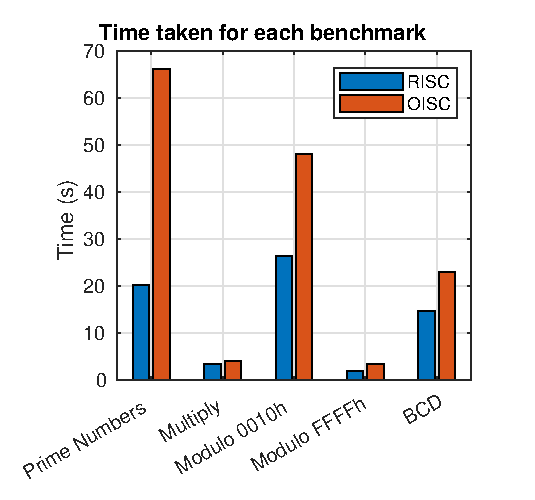
\includegraphics[width=\linewidth]{../tests/timing.eps}
	\captionof{figure}{Time taken perform each benchmark on FPGA at 1MHz clock.}
	\label{fig:timing}
\end{colfigure}

Results indicate that on average OISC takes about 71\% longer to execute same benchmark. This is close to results found with simulation. Prime number calculator have taken 3.26 times longer.

Benchmarks include:
\begin{description}
	\item[$\bullet$ Prime Numbers:] Calculate every prime number between 5 to 65536.  
	\item[$\bullet$ Multipy:] 16bit multiplication iterated 65536 times.
	\item[$\bullet$ Modulo 0010h:] 16bit \textit{0010h} modulo that operated on every number between 0 and 65536.
	\item[$\bullet$ Modulo FFFFh:] 16bit \textit{FFFFh} modulo that operated on every number between 0 and 65536.
	\item[$\bullet$ BDC:] Encoded 16bit binary to ASCII decimal number without printing.
\end{description}


\subsubsection{Program space}

Data collected from previous instruction composition results were also used to find effective program size.
Effective program size only includes instruction that been executed depending on argument, meaning that it does not fully represent complete function. A specific input to a function might cause branching and avoiding some function code, which would not be added to effective program size. In this test, the main objective is to look difference in instruction size required to execute the same function, therefore not representing full program size is irrelevant. 
\begin{colfigure}
	\centering
	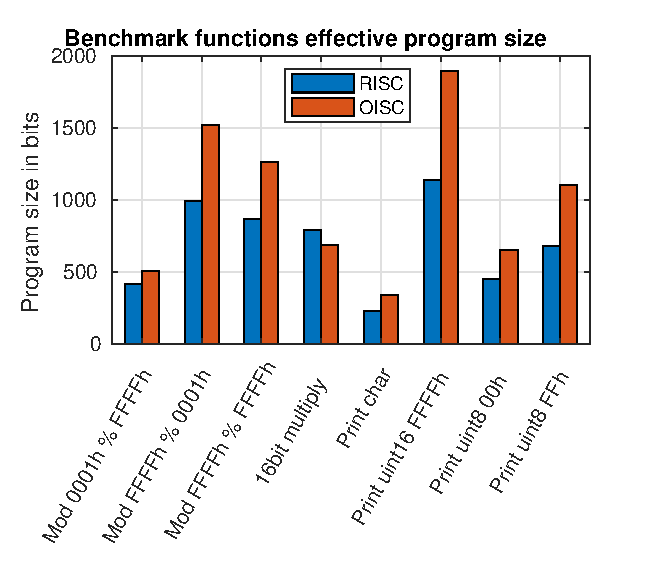
\includegraphics[width=\linewidth]{../tests/program_size.eps}
	\captionof{figure}{Bar graph showing effective size in bits each benchmark function is taking in program memeory.}
	\label{fig:program_size}
\end{colfigure}

Figure \ref{fig:program_size} represents an effective program size for each test function. On average, OISC instructions take 41.71\% more space which is to be expected.

\subsection{Maximum clock frequency}
In order to find maximum clock frequency, processors were loaded with basic print string function and 16bit multiplication. Then, frequency was constantly increased until resulting output though UART was not correct. 

In order to change clock frequency, three parameters were changed and HDL code resynthesised: 
\begin{description}
	\item[$\bullet$] \textbf{PLL frequency multiplier and divider:}
	PLL takes 50MHz clock and converts it to master clock $f_{mclk}$. Multiplier and divider values are used to adjust $f_{mclk}$.
	
	\item[$\bullet$] \textbf{UART frequency divider:}
	Division value was calculated as $D = \left \lfloor \frac{f_{mclk}}{4 f_{baud}} \right \rfloor$. UART rate was set to 9600 baud. UART module itself has four times oversample. 
\end{description}
Frequency was changed in 5MHz increments. 

Theoretical maximum frequency was found using Quartus Timing Analysis tool. Slow 1200mV 85$^{\circ}$C model was used. 

\begin{center}
	\begin{tabular}{ l | c | c  }
		     & Theoretical & Actual \\ \hline
		RISC & 114.08MHz & 75-70MHz \\ \hline
		OISC & 64.68MHz & 45-40MHz \\
	\end{tabular}
	\captionof{table}{Theoretical and actual maximum frequencies of both processors.}
	\label{tab:max_freq}
\end{center}

Theoretical and actual results show unexpected results shown in Table \ref{tab:max_freq}, RISC operated at about 40\% higher maximum frequency than OISC.

As explained in Subsection \ref{subsec:oisc_cell_issue}, OISC logic blocks has about twice less time for data propagation. Keeping that in mind, and assuming that latch propagation and register setup periods are insignificant to critical path of OISC logic block, maximum OISC frequency could be double as high as, reaching 80-90MHz. This also assumes that there is no other part of processor would have limit. Further timing analysis needs to be carried out to confirm this.

\subsection{Future work}

RISC has more sophisticated logic for various processor components. It is expected to see RISC having better results due to its higher optimisation. OISC should be implemented with multiple data \& instruction buses. This could be performed with minimal corrections on hardware, however would require many changes in assembly programs. \nameref{subsec:instr_comp} results show that OISC takes more instructions to store values in accumulators, which could benefit from multi-bus parallelisation. Adding a single additional bus should reduce benchmarks time by up to double, which would produce more comparable to RISC. In addition, multi-bus OISC can perform truly parallel programs assuming it has enough processor resources to perform operations (for example operate different ALU operations at the same time). This potentially would be dominant feature over RISC in time-sensitive programs, GPIO (General Purpose Input/Output) and interrupt handling. 

Additional buses would not greatly increase processor logic element size, especially when using interconnect optimisation techniques \autocite{1207041,6972455}. Matching processor complexity should also allow more fair and direct comparison specifically between two architectures. 

A number of other improvements and future research are proposed:
\begin{enumerate}
	\item Perform more tests on power analysis with different frequencies. Find the activity factor described in Subsection \ref{subsec:activity_factor}.
	\item Further investigate maximum frequency. Try to resolve OISC timing issue and repeat maximum frequency test. This would allow confirming or denying theorised higher frequency capabilities for OISC. 
	\item Design a higher level language compiler such as BASIC or C. This would allow performing more complicated programs which would more closely relate to microcontroller operations. However, OISC compiler would need extra optimisation layer to efficiently organise instructions.
	\item Compare proposed processor designs with other commercially available 8-bit processors such as Atmel AVR microcontrollers, Motorola 6800 family and Microchip PIC.
\end{enumerate}



	\section{Conclusion}\label{sec:conclusion}
	\iffalse
The final chapter is short and sweet, to the point:
 what did you really accomplish? 
 What significant result can you claim and how it differs from anything done before. 
 How well did you meet your goal? 
 Now step out one level, then another indicating the impact your work will have on the literature and on future endeavours.
 * Start with the specifics and end with the general.
 * Summarise key result; mention limitations, note anything unexpected.
\fi
	\vfill\pagebreak
	\printbibliography
	\onecolumn
	\section{Appendix}\label{sec:appendix}
	% !TeX root = index.tex

\subsection{Processor instruction set tables}\label{subsec:instruction_sets}
\arrayrulecolor{black}
\begin{longtable}[h!]{| l | p{.70\textwidth} | c |}
\caption{Instruction set for RISC processor. * Required immediate size in bytes}
\label{tab:risc_instructions}\\

\hline
\rowcolor[rgb]{0.82,0.82,0.82}
Instr. & Description & I-size *\\\hline
\endhead		

\arrayrulecolor{black}\hline
\endfoot

\multicolumn{3}{|c|}{
	\cellcolor[rgb]{0.7,0.7,1}\textit{2 register instructions}} \\\hline
\arrayrulecolor[rgb]{0.82,0.82,0.82}

MOVE & Copy value from one register to other & 0 \\\hline
ADD  & Arithmetical addition & 0 \\
SUB  & Arithmetical subtraction & 0  \\
AND  & Logical AND & 0 \\
OR   & Logical OR & 0 \\
XOR  & Logical XOR & 0 \\
MUL  & Arithmetical multiplication & 0 \\
DIV  & Arithmetical division (inc. modulo) & 0 \\


\arrayrulecolor{black}\hline
\multicolumn{3}{|c|}{
	\cellcolor[rgb]{0.7,0.7,1}\textit{1 register instructions}} \\
\hline\arrayrulecolor[rgb]{0.82,0.82,0.82}


COPY0 & Copy intimidate to a register 0 & 1 \\
COPY1 & Copy intimidate to a register 1 & 1 \\
COPY2 & Copy intimidate to a register 2 & 1 \\
COPY3 & Copy intimidate to a register 3 & 1 \\\hline

ADDC & Arithmetical addition with carry bit& 0 \\
ADDI & Arithmetical addition with immediate & 1 \\
SUBC & Arithmetical subtraction with carry bit & 0 \\
SUBI & Arithmetical subtraction with immediate & 1 \\\hline

ANDI & Logical AND with immediate & 1 \\
ORI  &  Logical OR with immediate & 1 \\
XORI &  Logical XOR with immediate & 1 \\\hline

CI0  & Replace intimidate value byte 0 for next instruction & 1 \\
CI1  & Replace intimidate value byte 1 for next instruction & 1 \\
CI2  & Replace intimidate value byte 2 for next instruction & 1 \\\hline

SLL  & Shift left logical & 1 \\
SRL  & Shift right logical & 1 \\
SRA  & Shift right arithmetical & 1 \\\hline

LWHI & Load word (high byte) & 3 \\
SWHI & Store word (high byte, reg. only) & 0 \\
LWLO & Load word (low byte) & 3 \\
SWLO & Store word (low byte, stores high byte reg.) & 3 \\\hline

INC  & Increase by 1 & 0 \\
DEC  & Decrease by 1 & 0 \\
GETAH& Get ALU high byte reg. (only for MUL \& DIV \& ROL \& ROR) & 0 \\
GETIF& Get interrupt flags & 0 \\\hline

PUSH & Push to stack & 0 \\
POP  & Pop from stack & 0 \\
COM  & Send/Receive to/from com. block & 1 \\\hline

BEQ  & Branch on equal & 3 \\
BGT  & Branch on greater than & 3 \\
BGE  & Branch on greater equal than & 3 \\
BZ   & Branch on zero & 2 \\

\arrayrulecolor{black}\hline
\multicolumn{3}{|c|}{
	\cellcolor[rgb]{0.7,0.7,1}\textit{0 register instructions}
} \\
\hline\arrayrulecolor[rgb]{0.82,0.82,0.82} 

CALL & Call function, put return to stack & 2 \\
RET  & Return from function & 0 \\
JUMP & Jump to address & 2 \\
RETI & Return from interrupt & 0 \\
INTRE& Set interrupt entry pointer & 2 \\\hline


\end{longtable}	

\arrayrulecolor{black}
\begin{longtable}[h!]{| l | p{0.8\textwidth} |}
	\caption{Instructions for OISC processor.}
	\label{tab:oisc_instructions}\\
	
	\hline 
	\rowcolor[rgb]{0.82,0.82,0.82}
	Name & Description \\\hline
	\endhead		
	
	\arrayrulecolor{black}\hline
	\endfoot
	
	\multicolumn{2}{|c|}{
		\cellcolor[rgb]{0.7,0.7,1}\textit{Destination Addresses}} \\\hline
	\arrayrulecolor[rgb]{0.82,0.82,0.82}
	
	ACC0 & Set ALU source A accumulator \\
	ACC1 & Set ALU source B accumulator \\\hline
	BR0  & Set Branch pointer register (low byte) \\
	BR1  & Set Branch pointer register (high byte) \\
	BRZ  & If source value is 0, set program counter to branch pointer \\\hline
	STACK& Push value to stack \\
	MEM0 & Set Memory pointer register (low byte) \\
	MEM1 & Set Memory pointer register (middle byte) \\
	MEM2 & Set Memory pointer register (high byte) \\
	MEMHI& Save high byte to memory at memory pointer \\
	MEMLO& Save low byte to memory at memory pointer \\\hline
	COMA & Set communication block address register \\
	COMD & Send value to communication block \\\hline
	REG0 & Set general purpose register 0 \\
	REG1 & set general purpose register 1 \\
	
	\arrayrulecolor{black}\hline
	\multicolumn{2}{|c|}{
		\cellcolor[rgb]{0.7,0.7,1}\textit{Source Addresses}} \\\hline
	\arrayrulecolor[rgb]{0.82,0.82,0.82}
	
	NULL & Get constant 0 \\
	ALU0 & Get value at ALU source A accumulator \\
	ALU1 & Get value at ALU source B accumulator \\\hline
	
	ADD  & Get Arithmetical addition of ALU sources \\
	ADDC & Get Arithmetical addition carry \\
	ADC  & Get Arithmetical addition of ALU sources and carry \\\hline
	
	SUB  & Get Arithmetical subtraction of ALU sources \\
	SUBC & Get Arithmetical subtraction carry \\
	SBC  & Get Arithmetical subtraction of ALU sources and carry \\\hline
	
	AND  & Get Logical AND of ALU sources \\
	OR   & Get Logical OR of ALU sources \\
	XOR  & Get Logical XOR of ALU sources \\\hline
	
	SLL  & Get ALU source A shifted left by source B \\
	SRL  & Get ALU source A shifted right by source B \\
	ROL  & Get rolled off value from previous SLL instance \\
	ROR  & Get rolled off value from previous SRL instance \\\hline
	
	MULLO& Get Arithmetical multiplication of ALU sources (low byte) \\
	MULHI& Get Arithmetical multiplication of ALU sources (high byte) \\
	DIV  & Get Arithmetical division of ALU sources \\
	MOD  & Get Arithmetical modulo of ALU sources \\\hline
	
	EQ   & Check if ALU source A is equal to source B \\
	GT   & Check if ALU source A is greater than source B \\
	GE   & Check if ALU source A is greater or equal to source B \\
	NE   & Check if ALU source A is not equal to source B \\
	LT   & Check if ALU source A is less than source B \\
	LE   & Check if ALU source A is less or equal to to source B \\\hline
	
	BR0  & Get Branch pointer register value (low byte) \\
	BR1  & Get Branch pointer register value (high byte) \\	
	PC0  & Get Program counter value (low byte) \\
	PC1  & Get Program counter value (high byte) \\\hline
	
	MEM0 & Get Memory pointer register value (low byte) \\
	MEM1 & Get Memory pointer register value (middle byte) \\
	MEM2 & Get Memory pointer register value (high byte) \\
	MEMHI& Load high byte from memory at memory pointer \\
	MEMLO& Load low byte from memory at memory pointer \\\hline
	
	STACK& Pop value from stack \\
	ST0  & Get stack address value (low byte) \\
	ST1  & Get stack address value (high byte) \\
	
	COMA & Get communication block address register value \\
	COMD & Read value from communication block \\\hline
	
	REG0 & Get value from general purpose register 0 \\
	REG1 & Get value from general purpose register 1 \\
	
\end{longtable}	


	
\end{document}